\chapter{Testy wydajnościowe}

\section{Wstęp}
 
W~poniższym rozdziale przedstawione zostaną wyniki testów wydajnościowych implementacji algorytmów
opisanych w~poprzedniej części pracy (poza algorytmem \emph{two-stage}, który został rozwinięty
i~poprawiony przez \emph{improved two-stage}). Implementacja w~języku \texttt{Java} została oparta
o~oryginalny kod, udostępniony przez autorów. Podstawą implementacji metody \emph{improved
two-stage} był kod algorytmu \emph{divsufsort} napisany przez Yutę Moriego [\ref{libdivsufsort}].

Algorytmy tworzenia tablic sufiksów zaimplementowane zostały w~ten sposób, żeby na wejściu
przyjmowały sekwencje liczb całkowitych typu \texttt{int} zajmujących w~języku \texttt{Java} 4
bajty. Spowodowało to zwiększenie złożoności pamięciowej algorytmów (wartości podane w~tabeli
\ref{tab:alg} zakładały wejście w~postaci sekwencji jednobajtowych elementów). Powodem zwiększenia
rozmiaru pojedynczego elementu wejściowego było umożliwienie tworzenia tablic sufiksów dla sekwencji
symboli z~alfabetów o~dużym rozmiarze. Nie jest to jednak możliwe w~praktyce w~przypadku wszystkich
algorytmów; rzeczywista złożoność pamięciowa implementacji wybranych metod oraz ich zależność od
rozmiaru alfabetu wejściowego opisane zostały w~tabeli \ref{tab:alg-impl}. Testowane implementacje
algorytmów \emph{bpr}, \emph{deep-shallow} i~\emph{qsufsort} dla zaoszczędzenia pamięci nadpisywały
ciąg wejściowy. Na potrzeby testów wydajnościowych zaimplementowano również naiwny algorytm
tworzenia tablic sufiksów opierający się o~zwykły algorytm sortujący \emph{quicksort}. W~dalszej
części rozdziału metoda naiwna nazywana będzie \emph{naive sort} lub NS.

Wykonane testy algorytmów można podzielić na dwie główne kategorie: testy na wejściu generowanym
losowo, oraz testy na wejściu wczytywanym z~plików. Testy drugiego typu wykonywane były na kilku
różnych maszynach wirtualnych:

\begin{itemize}
    \item maszyna Java HotSpot 64-Bit Server VM 11.0-b16 firmy Sun Microsystems, oznaczana w~dalszej części pracy jako \texttt{sun},
    \item maszyna IBM J9 VM 2.4 firmy IBM, oznaczana w~dalszej części pracy jako \texttt{ibm},
    \item BEA JRockit(R) R27.5.0-110\_o-99226-1.6.0\_03 firmy BEA (aktualnie przejęta przez Oracle), oznaczana w~dalszej części pracy jako \texttt{jrockit},
    \item Apache Harmony DRLVM 11.2.0 tworzona przez Apache Software Foundation, oznaczana w~dalszej części pracy jako \texttt{harmony}.
\end{itemize} 

\begin{table}[ht]
    \begin{center}        
        \begin{tabular}{l r r}
         \toprule
            Nazwa & Złożoność pamięciowa \\
         \midrule
            \emph{skew} & $16n$  \\
            \emph{bpr} & $4|\Sigma|^3+12n$ \\ 
            \emph{deep-shallow} & $4|\Sigma|^2+(x+8)n$  \\
            \emph{divsufsort} & $4|\Sigma|^2+8n$ \\
            \emph{qsufsort} & $8n$ \\
            \emph{naive sort} & $8n$ \\
        \bottomrule
        \end{tabular}
    \end{center}                         
    \caption{Zaimplementowane algorytmy tworzenia tablic sufiksów. Parametr $n$ oznacza długość wejścia, 
    parametr $|\Sigma|$ oznacza wielkość alfabetu sekwencji wejściowej. Algorytm \emph{deep-shallow} wymaga
    alfabetu o~rozmiarze nie większym niż 256, zużycie pamięci przez ten 
    algorytm zależy od wielkości budowanego drzewa \emph{blind trie}, które maksymalnie może zawierać $n$ elementów. Rozmiar jednego elementu drzewa wynosi $x=48$ bajtów na 64-bitowej maszynie wirtualnej firmy Sun.
    Algorytmy \emph{bpr} i~\emph{divsufsort} nie mają sztywnych ograniczeń na rozmiar 
    alfabetu, ale ze względu na wydajność nie powinny być używane na dużych alfabetach.}%
    \label{tab:alg-impl}
\end{table}
	
\noindent
Testy przeprowadzone zostały na kilku komputerach testowych o~następujących parametrach:
\begin{itemize}
    \item dwurdzeniowy procesor Athlon 5200 o~prędkości 2.6 GHz, 64-bitowy system operacyjny OpenSuSE, jądro w~wersji 2.6.22.19-0.2-default,
    \item czterordzeniowy procesor Intel Xeon x3230 o~prędkości 2.66 GHz, 64-bitowy system operacyjny OpenSuSE, wersja jądra 2.6.22.19-0.2-default,
    \item jednordzeniowy Intel Pentium 4 o~prędkości 3 GHz, 32-bitowy system operacyjny Windows XP.
\end{itemize}
	
\noindent
Wszystkie obliczenia przeprowadzone zostały z~parametrami maszyn wirtualnych
odpowiadającym opcjom ,,\texttt{-Xmx2g -server}'' -- zwiększają one maksymalny rozmiar 
sterty do 2Gb, a~maszyna wirtualna pracuje w~trybie ,,serwerowym'' (agresywna optymalizacja JIT).
	
Czas działania algorytmów mierzony był przez klasę uruchamiającą testy, poprzez liczenie różnicy
wartości zwracanych przez metodę \texttt{System.currentTimeMillis()} przed i~po obliczeniach
(tzw.~\emph{wall time}). Do mierzenia zużycia pamięci wykorzystano specjalnie w~tym celu napisany
aspekt [\ref{aspectj}]. Mierzone było zużycie pamięci wewnątrz wirtualnej maszyny na początku
działania algorytmu, pod jego koniec oraz po zakończeniu wybranych metod wewnątrz klas. Mierzenie
zużycia pamięci w~języku \texttt{Java} jest trudne, bowiem maszyna wirtualna nie pozwala na dokładne
oszacowanie wszystkich dokonanych alokacji pamięci. Do celów testowych posłużono się programowaniem
aspektowym i~,,wpleciono'' (\english{code weaving}) dynamiczne instrukcje mierzące różnicę
w~aktualnej ilości zaalokowanej pamięci względem startu algorytmu. Nie jest to oszacowanie idealne,
ale pozwala na zgrubne stwierdzenie ile pamięci zużywa dany algorytm.

Test na jednej instancji wejścia (pliku lub wygenerowanej sekwencji o~ustalonych parametrach)
powtarzany był 10 razy, a~jego wynikiem jest średnia z~zebranych pomiarów. Testy których wyniki
zbierano poprzedzano kilkoma uruchomieniami algorytmu. Celem tego zabiegu było wyeliminowanie błędów
pomiarowych wynikających z~wolniejszego działania kodu, który nie został skompilowany do kodu
natywnego przez maszynę wirtualną. Testy na wejściu generowanym losowo były poprzedzone 10 rundami
,,rozgrzewki", natomiast przed testem na wejściu wczytywanym z~pliku algorytm uruchamiany był 5
razy.
	
W~dalszej części rozdziału prezentowane są wyniki pochodzące z~pomiarów na komputerze z~procesorem
Xeon x3230. Wyniki z~pozostałych maszyn są niemal identyczne pod względem porównywania i~rankingu
algorytmów, dlatego też w wielu miejscach je pominięto (wszystkie wyniki są na dołączonej do pracy
płycie CD). Samo porównanie efektywności wykonania programów w różnych maszynach wirtualnych
znajduje się w rozdziale \ref{sect:vms}.


\section{Testy wydajnościowe na losowo generowanym wejściu}

Celem testów na losowo generowanym wejściu jest zbadanie rzeczywistej zależności algorytmów od
długości wejścia, wielkości alfabetu oraz średniego \emph{lcp} ciągu wejściowego. Testy
przeprowadzono tylko na jednej maszynie wirtualnej (\texttt{sun}). Ziarno generatora liczb losowych
otrzymywało identyczną wartość przed testem każdego algorytmu by zapewnić powtarzalność wyników.
	
	
\subsection{Wejście o~zmiennej długości i~stałej wielkości alfabetu}

Testy algorytmów na losowym wejściu o~zmiennej długości i~stałej wielkości alfabetu powtórzono trzy
razy. Każdy test wykonany był dla wejścia generowanego z~alfabetu wielkości 4,100 i~255 elementów.
Rysunek \ref{rys:random-input-lcp} przedstawia średnią wartość \emph{lcp} generowanych ciągów
wejściowych. Z~rysunku wynika, że wartość średniego \emph{lcp} jest mniej więcej odwrotnie
proporcjonalna do wielkości alfabetu.
		
Rysunki \ref{rys:random-input-time-4} i~\ref{rys:random-input-memory-4} przedstawiają czas działania
algorytmów oraz zużycie pamięci dla alfabetu wielkości 4. Algorytmy \emph{qsufsort} i~\emph{naive
sort} uzyskały najlepszy wynik złożoności pamięciowej. Zgodnie z~przewidywaniami, algorytmy
\emph{skew} i~\emph{deep shallow} wypadł najgorzej w~tej kwestii. Najszybszym algorytmem okazał się
być algorytm \emph{bpr}. Wyraźnie wolniejsze od pozostałych algorytmów są algorytmy \emph{skew}
i~\emph{naive sort}.


\begin{figure}[t]
       \begin{center}
            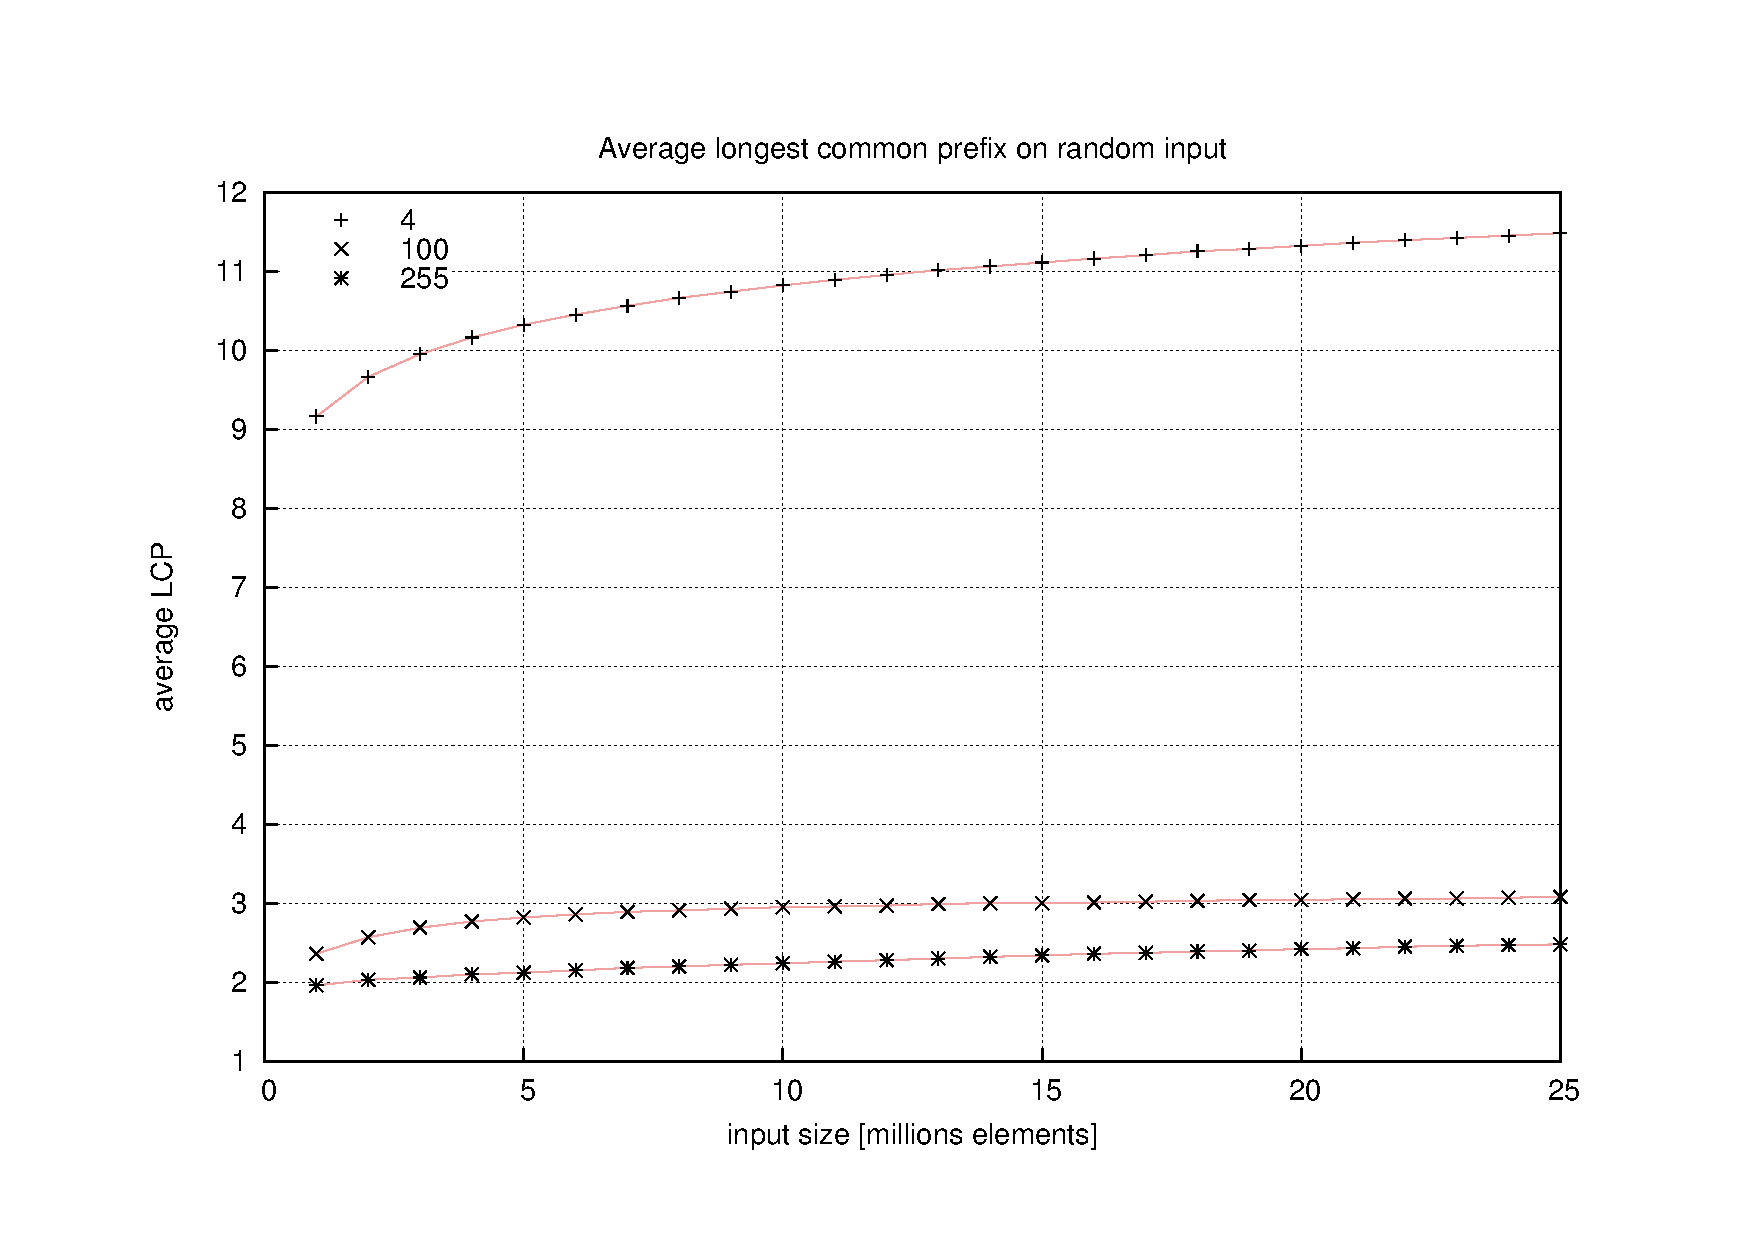
\includegraphics[width=\linewidth]{figures/results/random-input-lcp}
        \end{center}
    \caption{Średnie \emph{lcp} w~zależności od długości wejścia dla alfabetów o wielkości 4, 100 i~255 symboli.}%
    \label{rys:random-input-lcp}
\end{figure}

\begin{figure}[tp]
    \begin{center}
          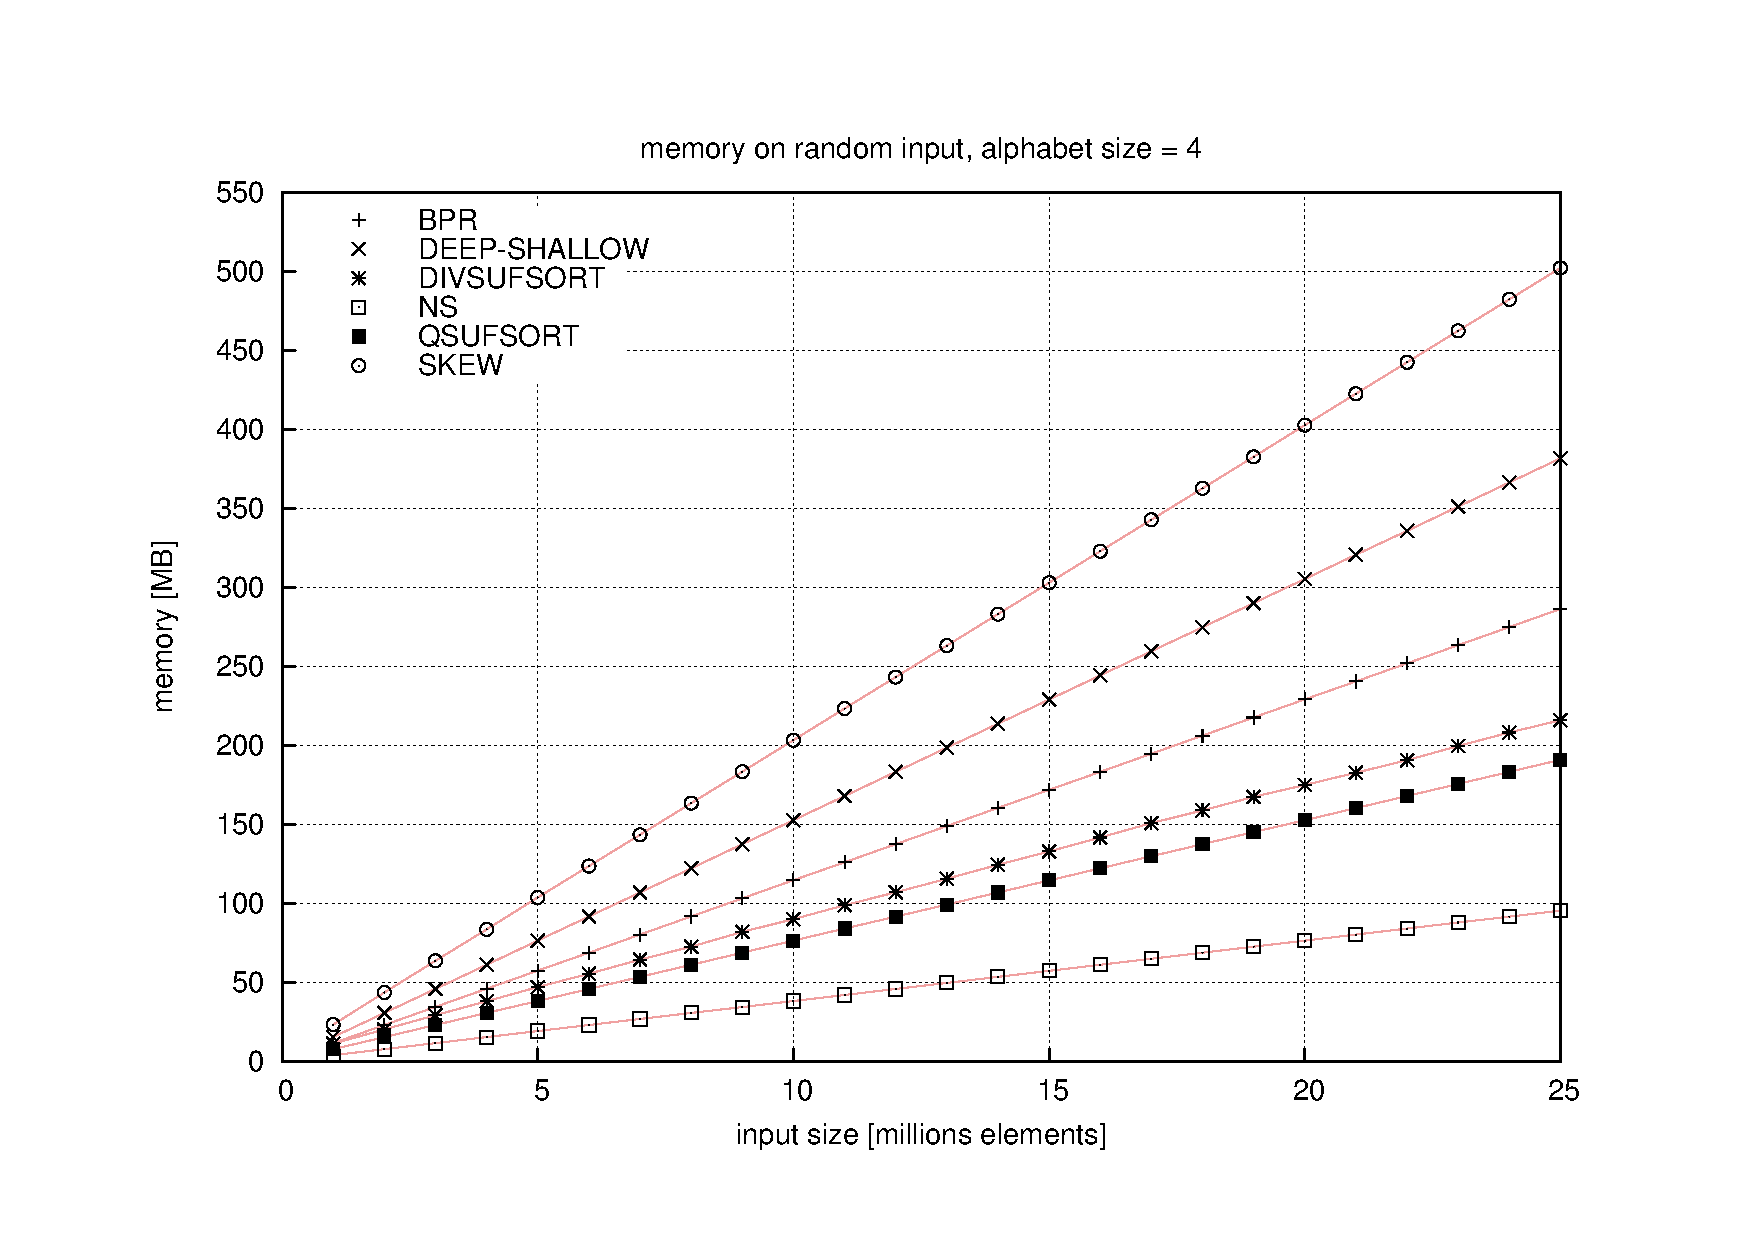
\includegraphics[width=\linewidth]{figures/results/random-input-memory-4}
    \end{center}
    \caption{Zużycie pamięci w~zależności od długości wejścia generowanego z~alfabetu wielkości 4.}%
    \label{rys:random-input-memory-4}
\end{figure}

%TODO wyniki zuzycia pamieci przez naive sort wskazuja na zaniżone wyniki pomiarów -- powinny być podobne wartości jak dla algorytmu qsufsort.
\begin{figure}[tp]
       \begin{center}
            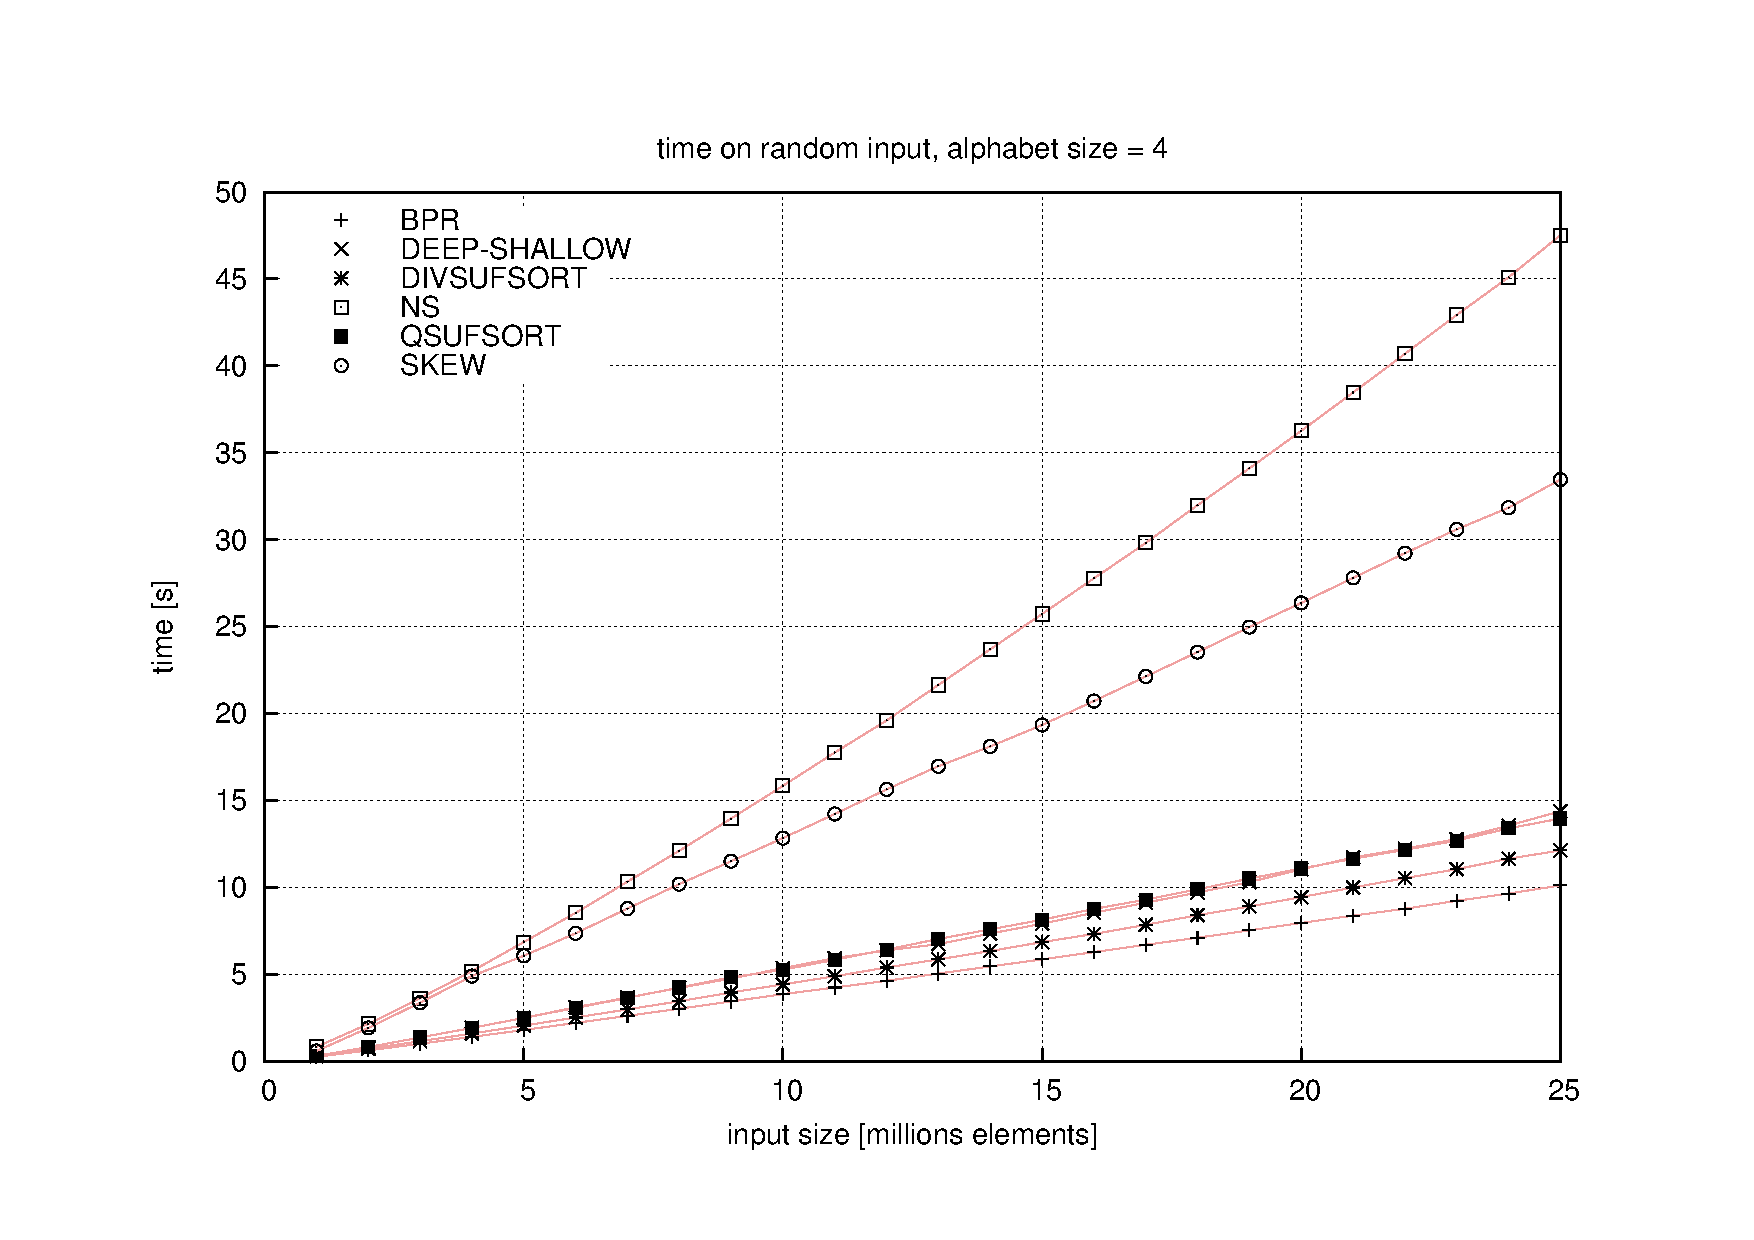
\includegraphics[width=\linewidth]{figures/results/random-input-time-4.pdf}
        \end{center}        
    \caption{Czas działania algorytmów w~zależności od długości wejścia generowanego z~alfabetu wielkości 4.}%
    \label{rys:random-input-time-4}
\end{figure}

\begin{figure}[tp]
   \begin{center}
      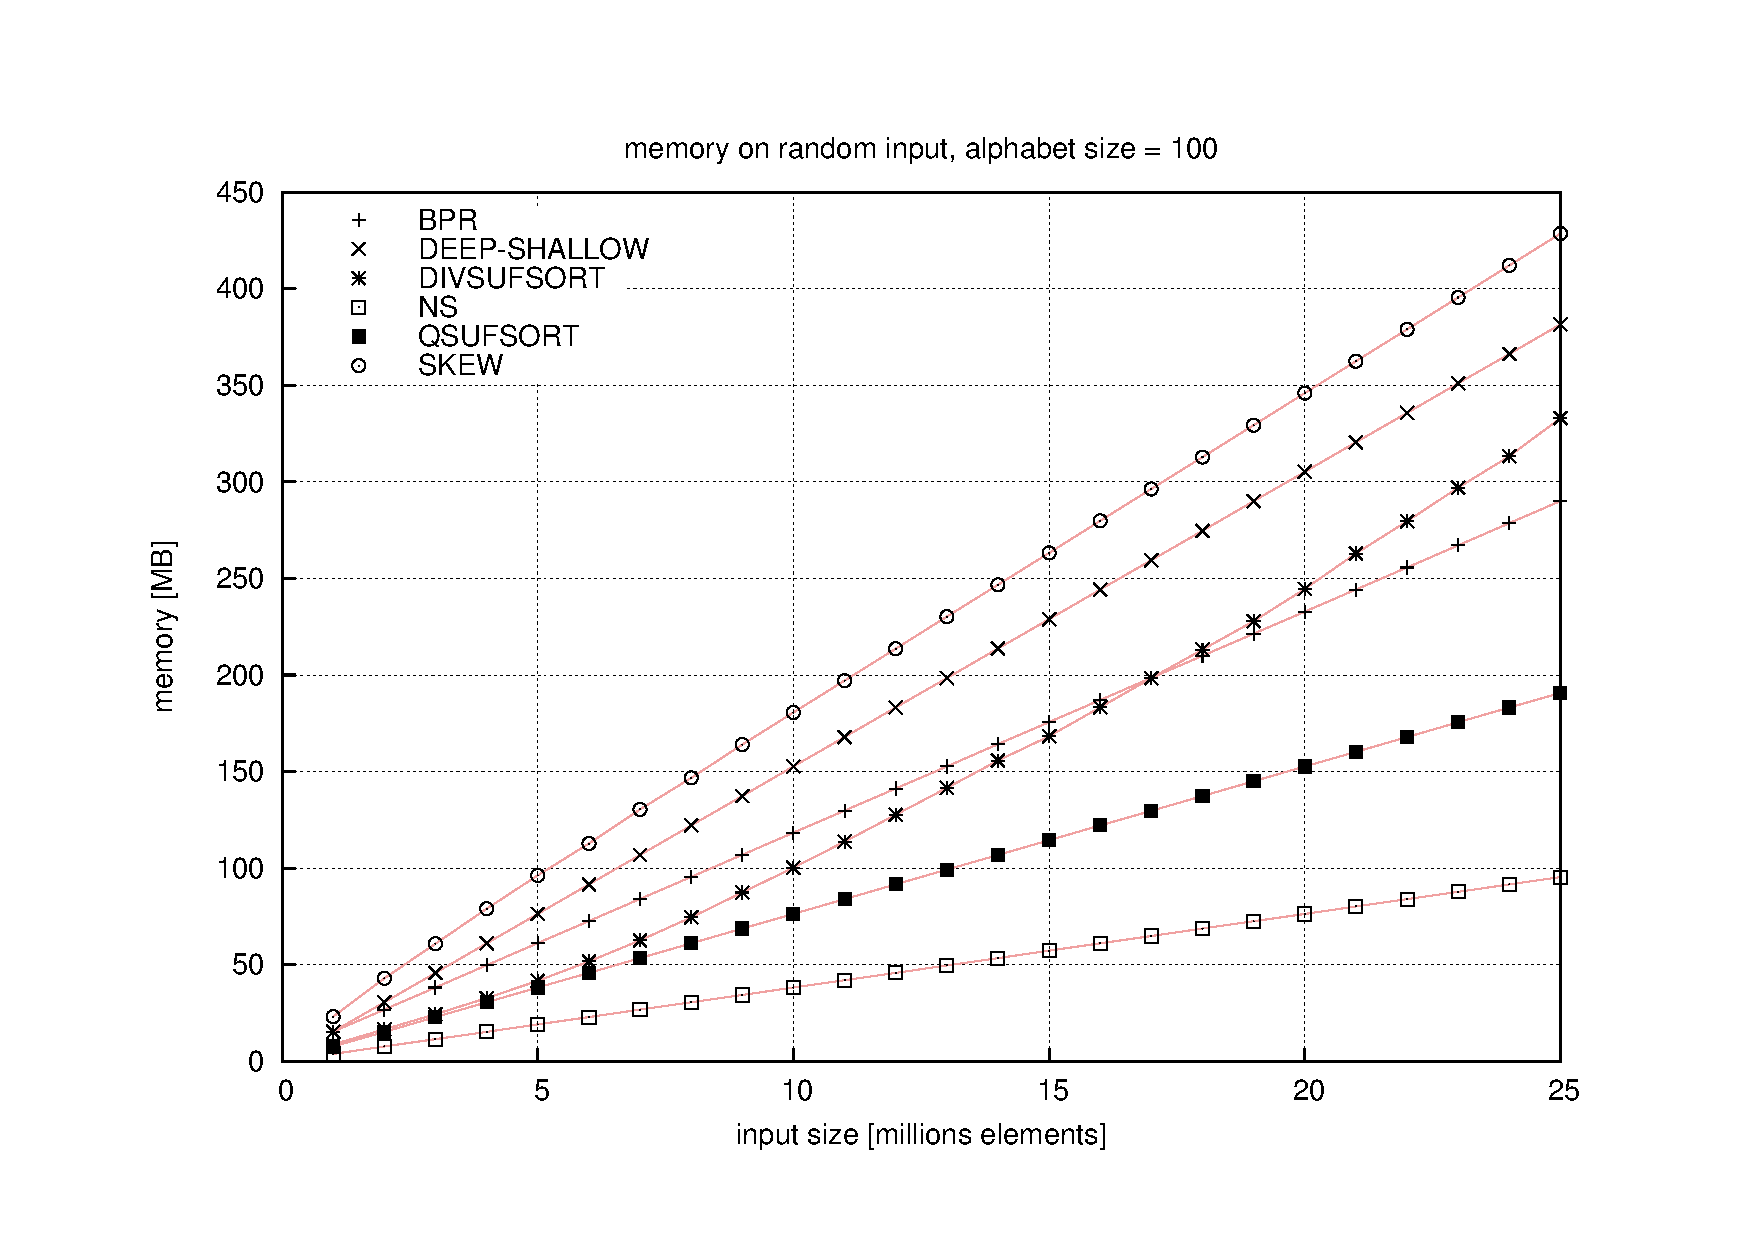
\includegraphics[width=\linewidth]{figures/results/random-input-memory-100.pdf}
    \end{center}        
    \caption{Zużycie pamięci w~zależności od długości wejścia generowanego z~alfabetu wielkości 100.}%
    \label{rys:random-input-memory-100}
\end{figure}

% nie wiem jak wyjaśnić zwiekszone zuzycie pamieci przez algorytm divsufsort
Wyniki testów wejścia generowanego z~alfabetu wielkości 100 przedstawione są na rysunku
\ref{rys:random-input-time-100} i~\ref{rys:random-input-memory-100}.
Rezultaty testu czasu działania algorytmu są niemal identyczne jak poprzedniego. Jedyną różnicą jest
to, że algorytm \emph{bpr} nie uzyskał najlepszego wyniku lecz znalazł się wśród kilku algorytmów
uzyskujących bardo dobry wynik, zajął również więcej pamięci.

\begin{figure}[tp]
   \begin{center}
        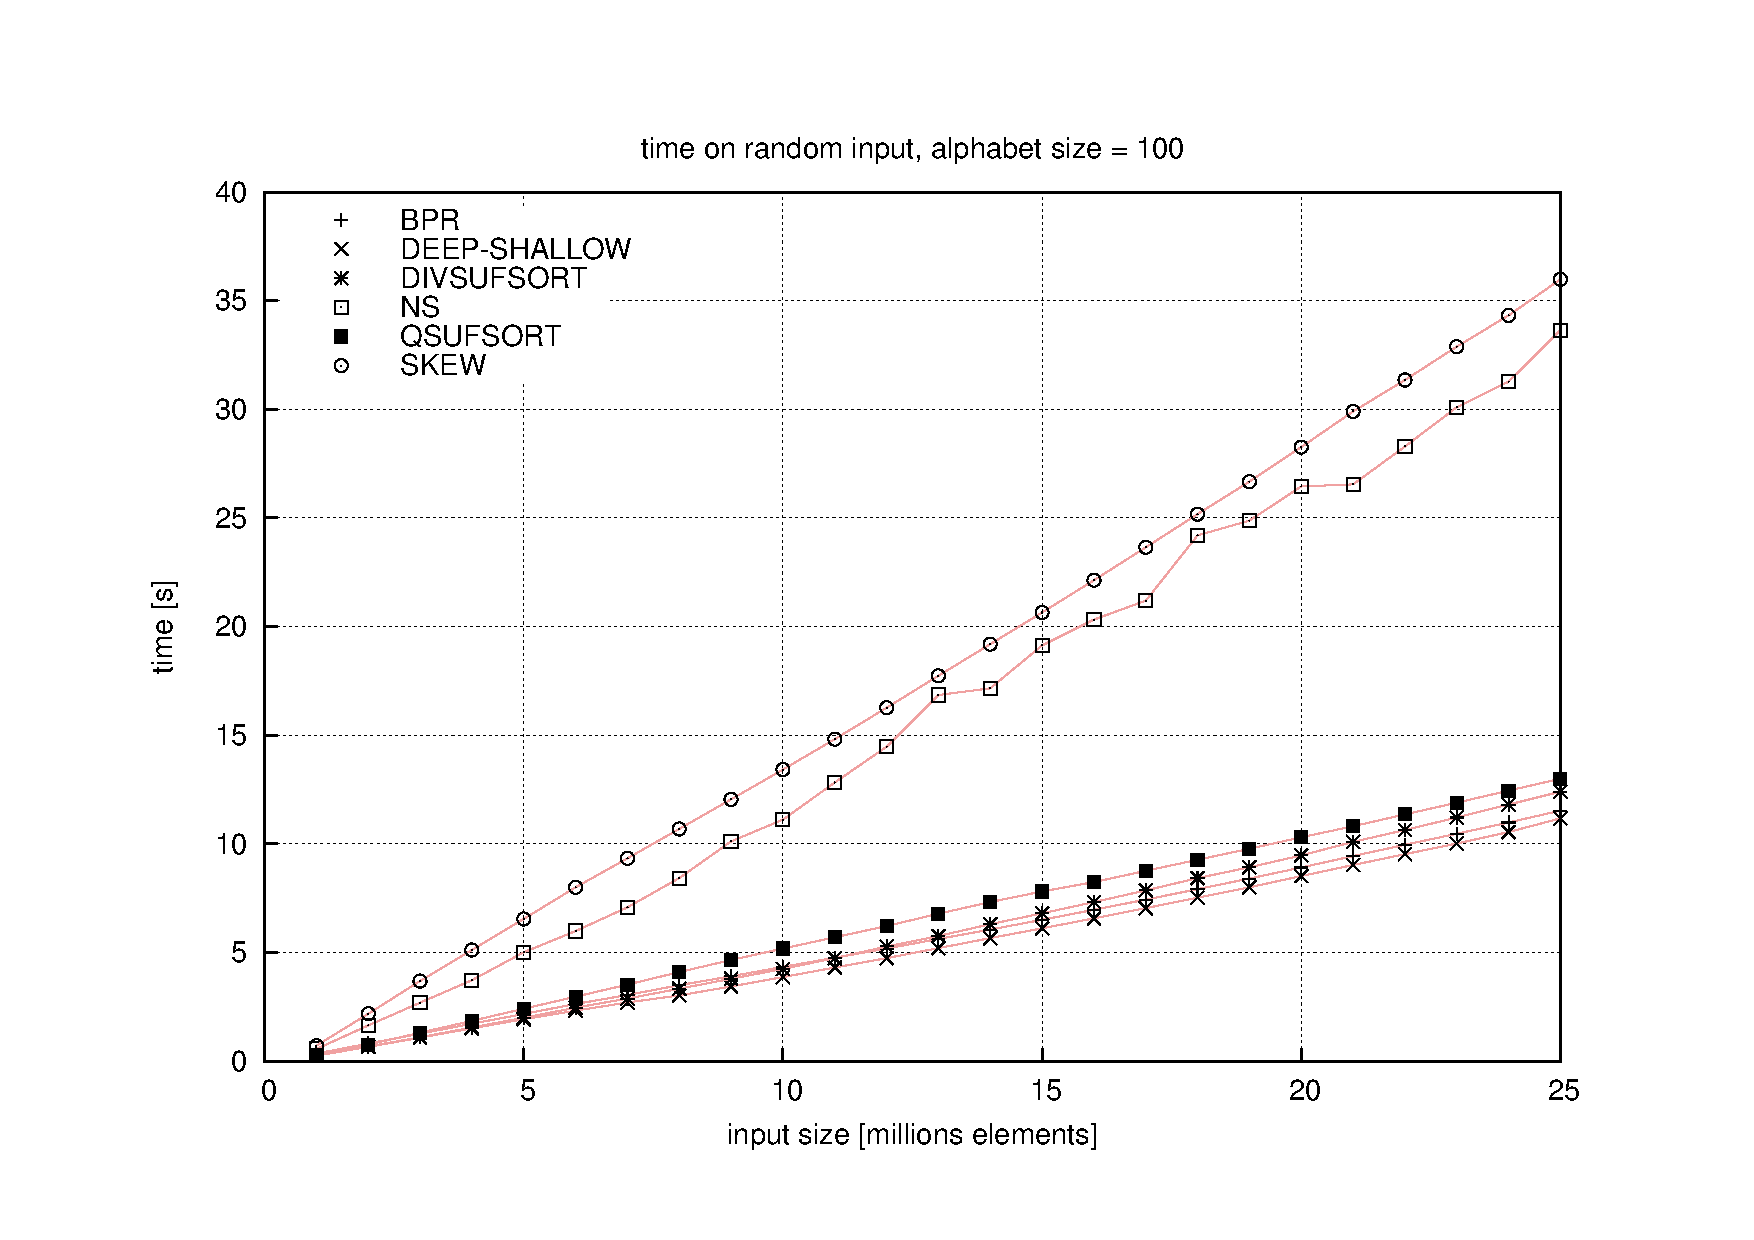
\includegraphics[width=\linewidth]{figures/results/random-input-time-100.pdf}
    \end{center}        
    \caption{Czas działania algorytmów w~zależności od długości wejścia generowanego z~alfabetu wielkości 100.}%
    \label{rys:random-input-time-100}
\end{figure} 

Rysunki \ref{rys:random-input-time-255} i~\ref{rys:random-input-memory-255} prezentują wyniki testów
wejścia generowanego z~alfabetu wielkości 255. Wynik tego testu są również podobne do poprzedników.
Algorytm \emph{bpr} uzyskał jeszcze gorszy wynik niż w~poprzednich testach, zajął więcej pamięci
i~działał wolniej od większości algorytmów.

\begin{figure}[tp]
       \begin{center}
          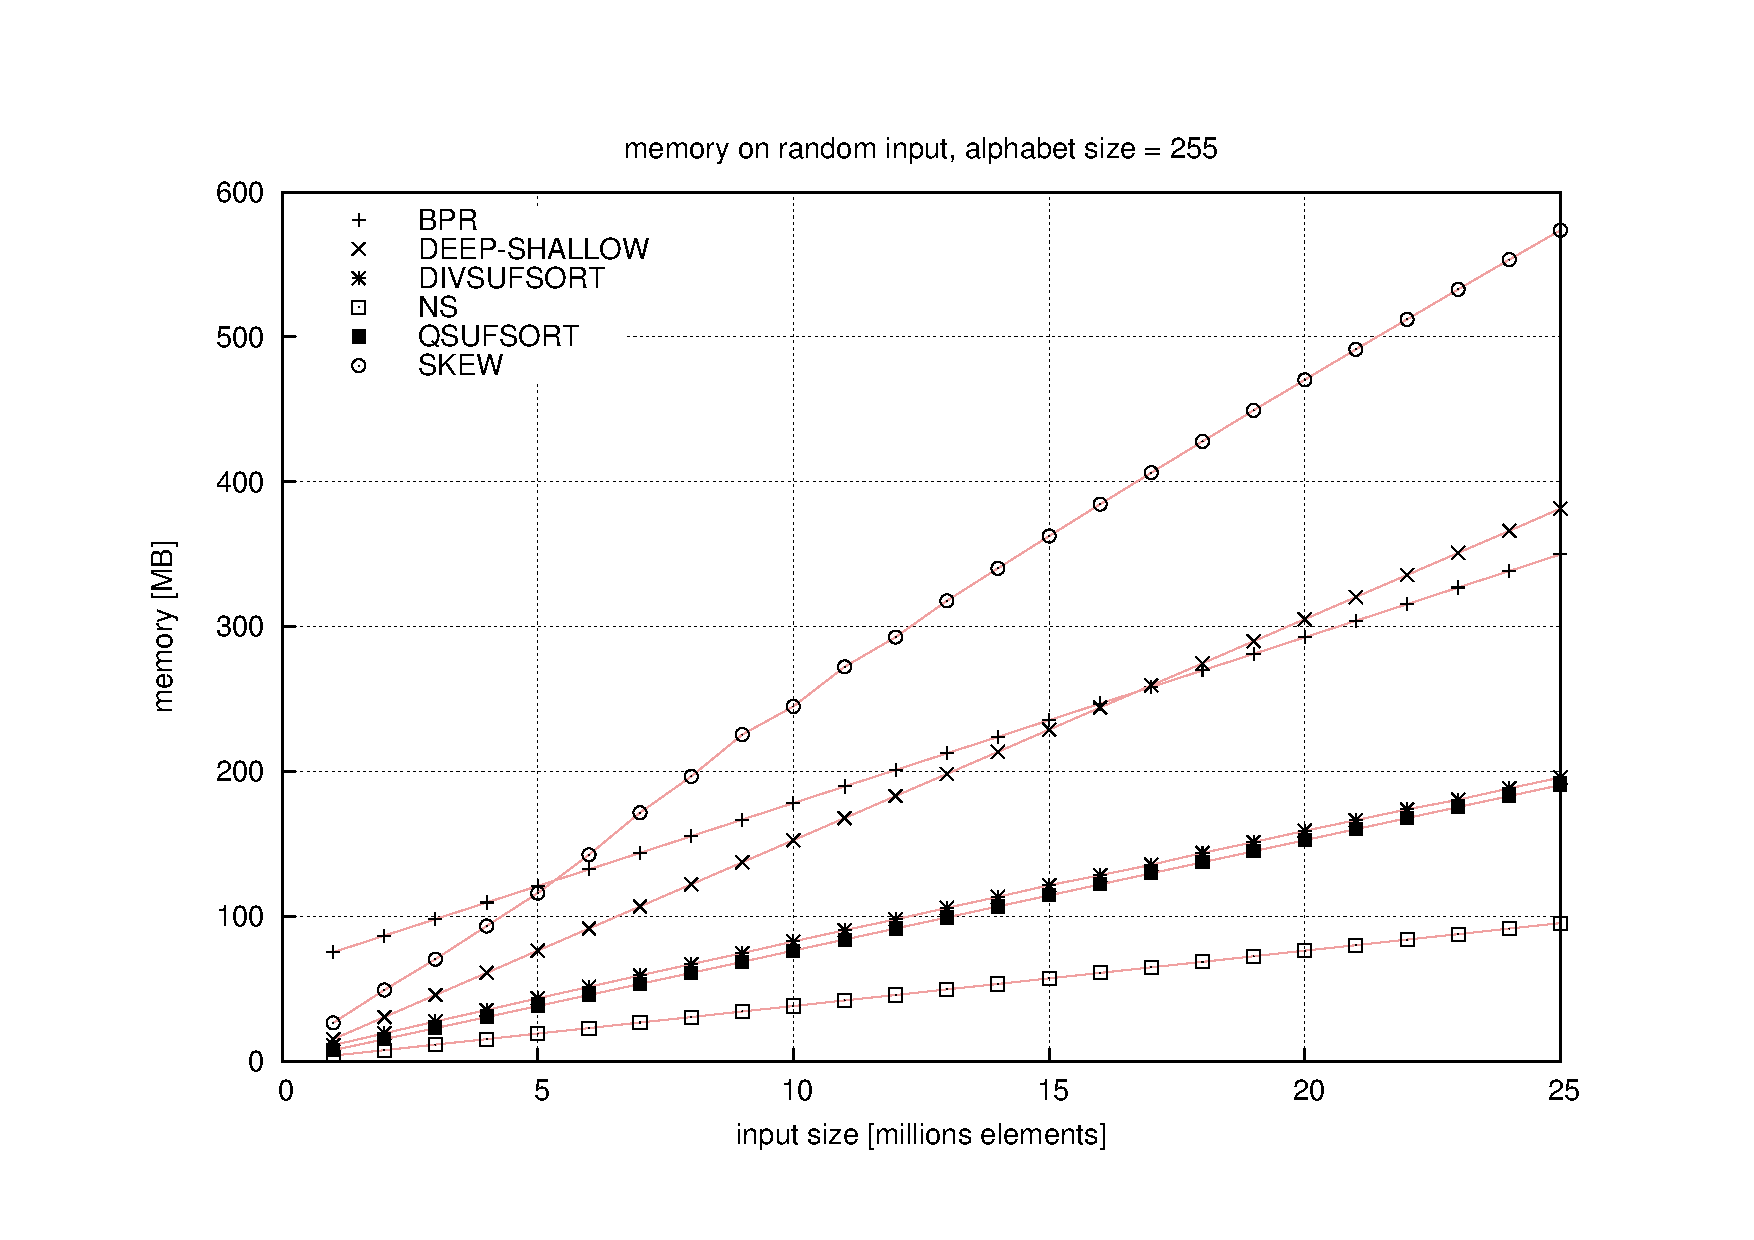
\includegraphics[width=\linewidth]{figures/results/random-input-memory-255.pdf}
        \end{center}        
    \caption{Zużycie pamięci w~zależności od długości wejścia generowanego z~alfabetu wielkości 255.}%
    \label{rys:random-input-memory-255}
\end{figure}

\begin{figure}[tp]
       \begin{center}
            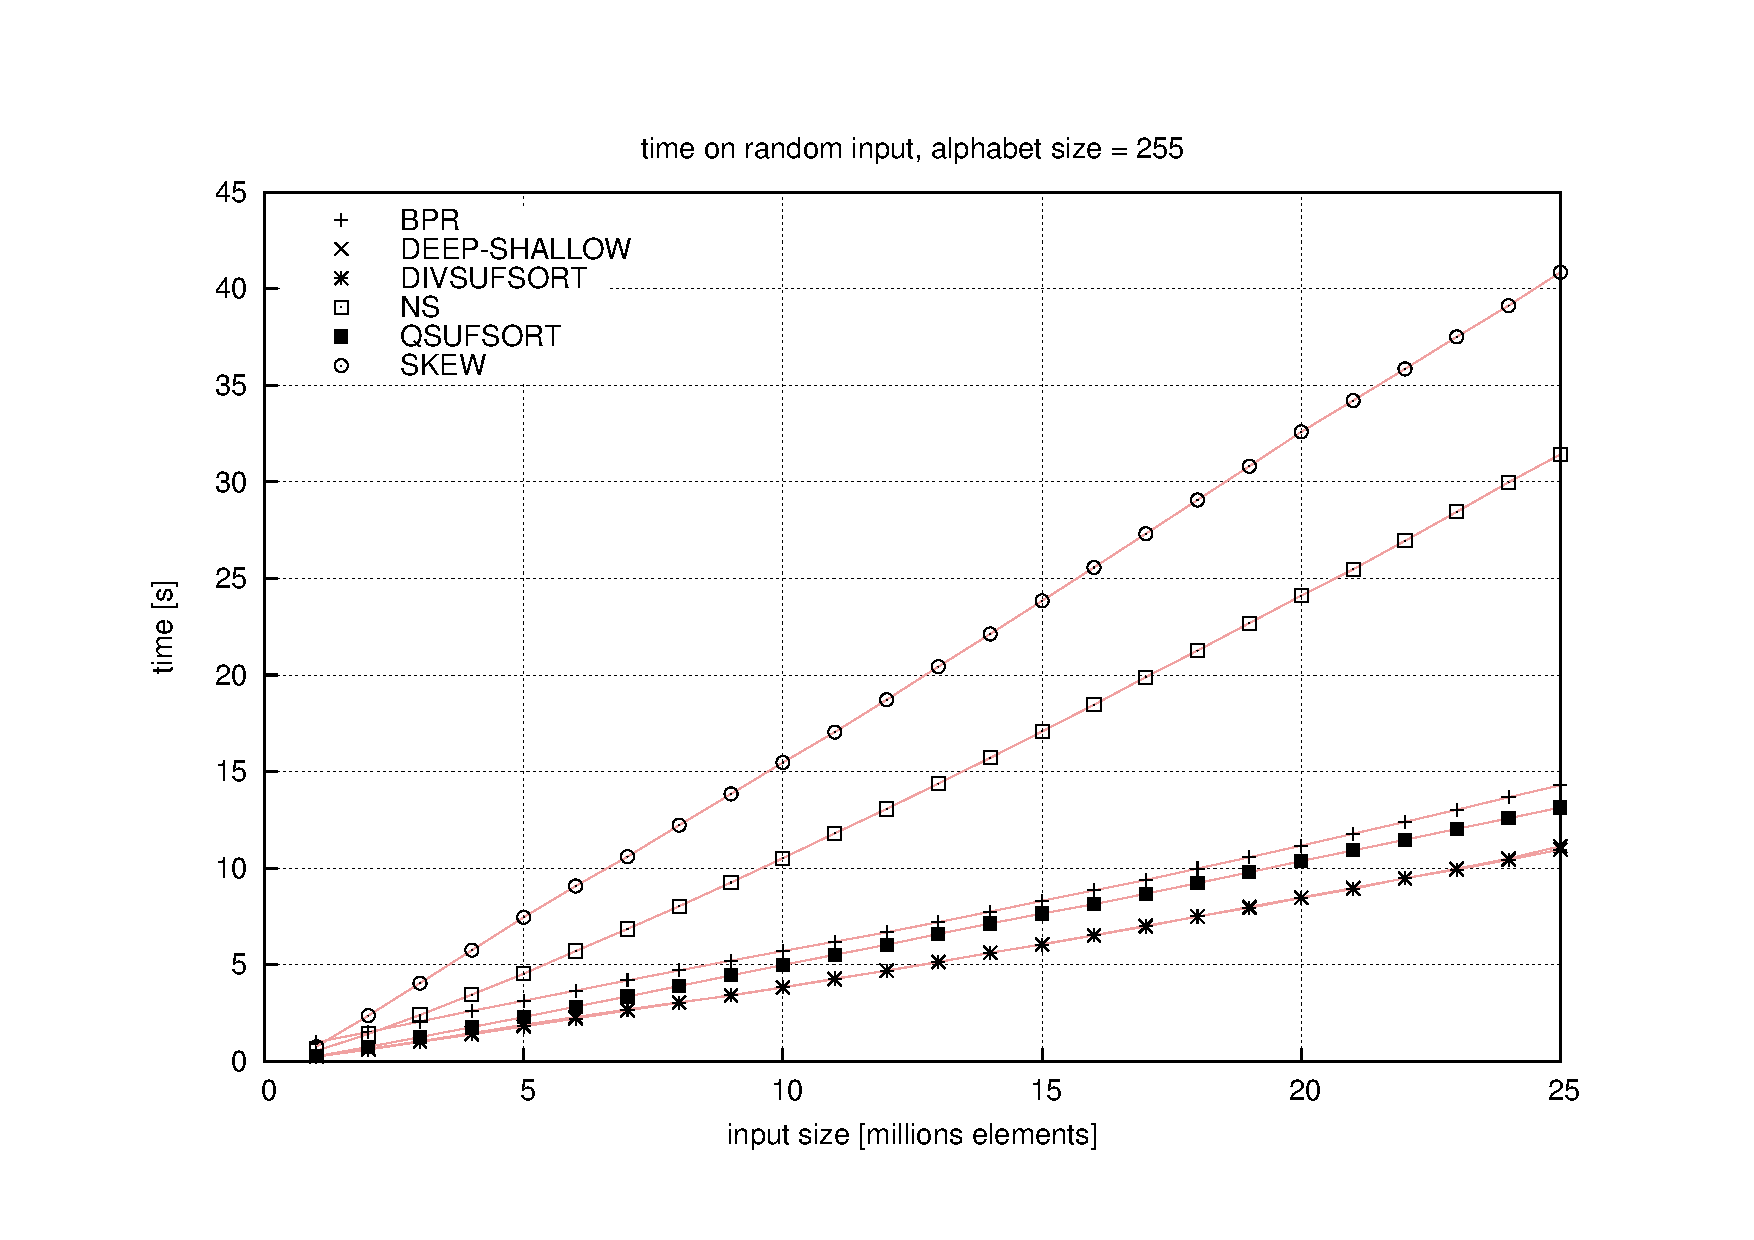
\includegraphics[width=\linewidth]{figures/results/random-input-time-255.pdf}
        \end{center}        
    \caption{Czas działania algorytmów w~zależności od długości wejścia generowanego z~alfabetu wielkości 255.}%
    \label{rys:random-input-time-255}
\end{figure} 


\subsection{Wejście o~stałej długości i~zmiennej wielkości alfabetu}

Wejście generowane na potrzeby testu miało długość 5\,000\,000 elementów. Wykres
\ref{rys:random-alphabet-lcp} przedstawia średnie \emph{lcp} wygenerowanego wejścia w~zależności od
wielkości alfabetu. Wykres \ref{rys:random-alphabet-time} przedstawia czasy działania algorytmów na
generowanym wejściu.

Wyniki testu pokazują które algorytmy zależą od średniego \emph{lcp} i~wielkości alfabetu sekwencji
wejściowej. Algorytm \emph{bpr} jest tego najlepszym przykładem -- im większa jest jedna z~tych
wartości, tym gorzej sobie radzi. Algorytm \emph{skew} uzyskuje lepsze wyniki dla sekwencji
o~większej wartości średniego \emph{lcp}. Pozostałe algorytmy nie wykazują większej zależności
pomiędzy czasem ich działania a~wielkością alfabetu i~średnim \emph{lcp}.
		
\begin{figure}[p]
       \begin{center}
            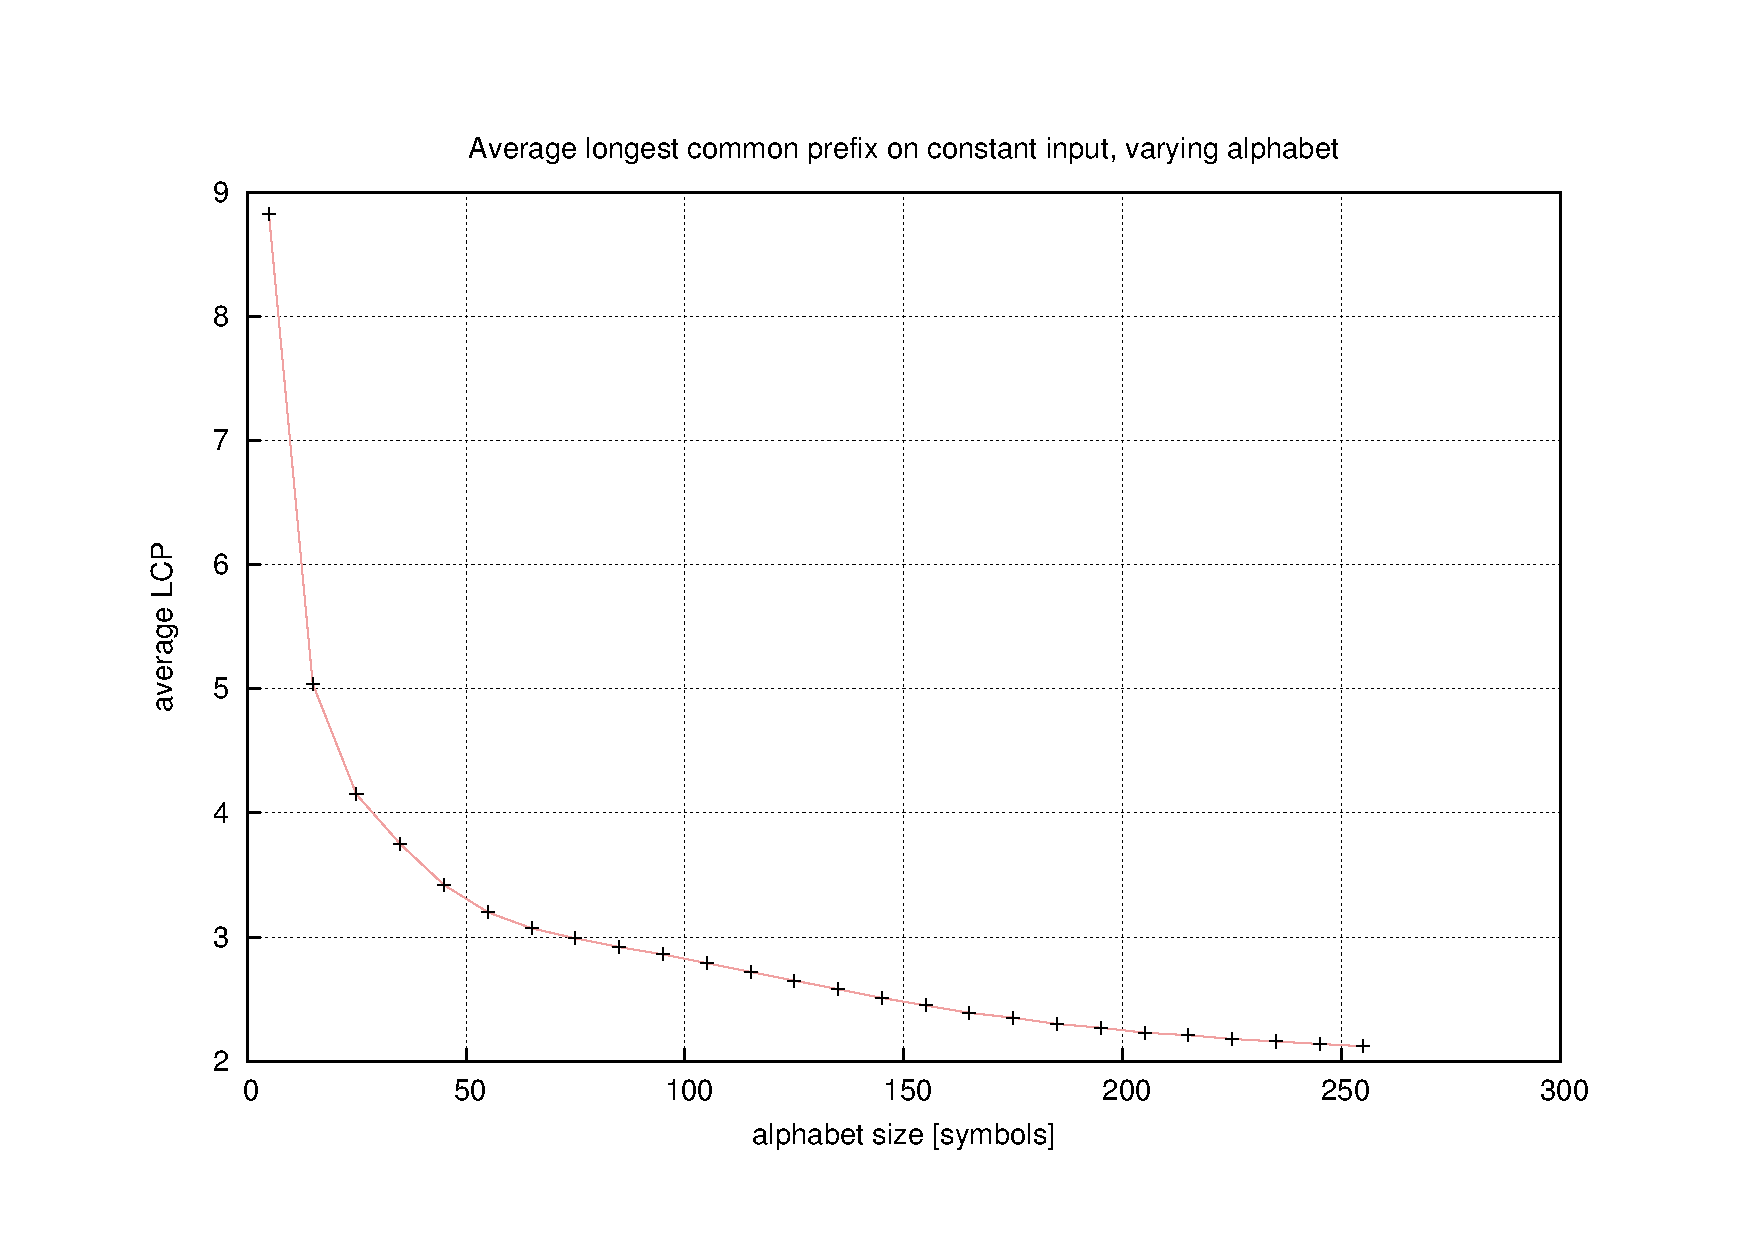
\includegraphics[width=\linewidth]{figures/results/random-alphabet-lcp.pdf}
        \end{center}        
    \caption{Średnie \emph{lcp} generowanego wejścia w~zależności od wielkości alfabetu.}%
    \label{rys:random-alphabet-lcp}
\end{figure}

\begin{figure}[p]
       \begin{center}
            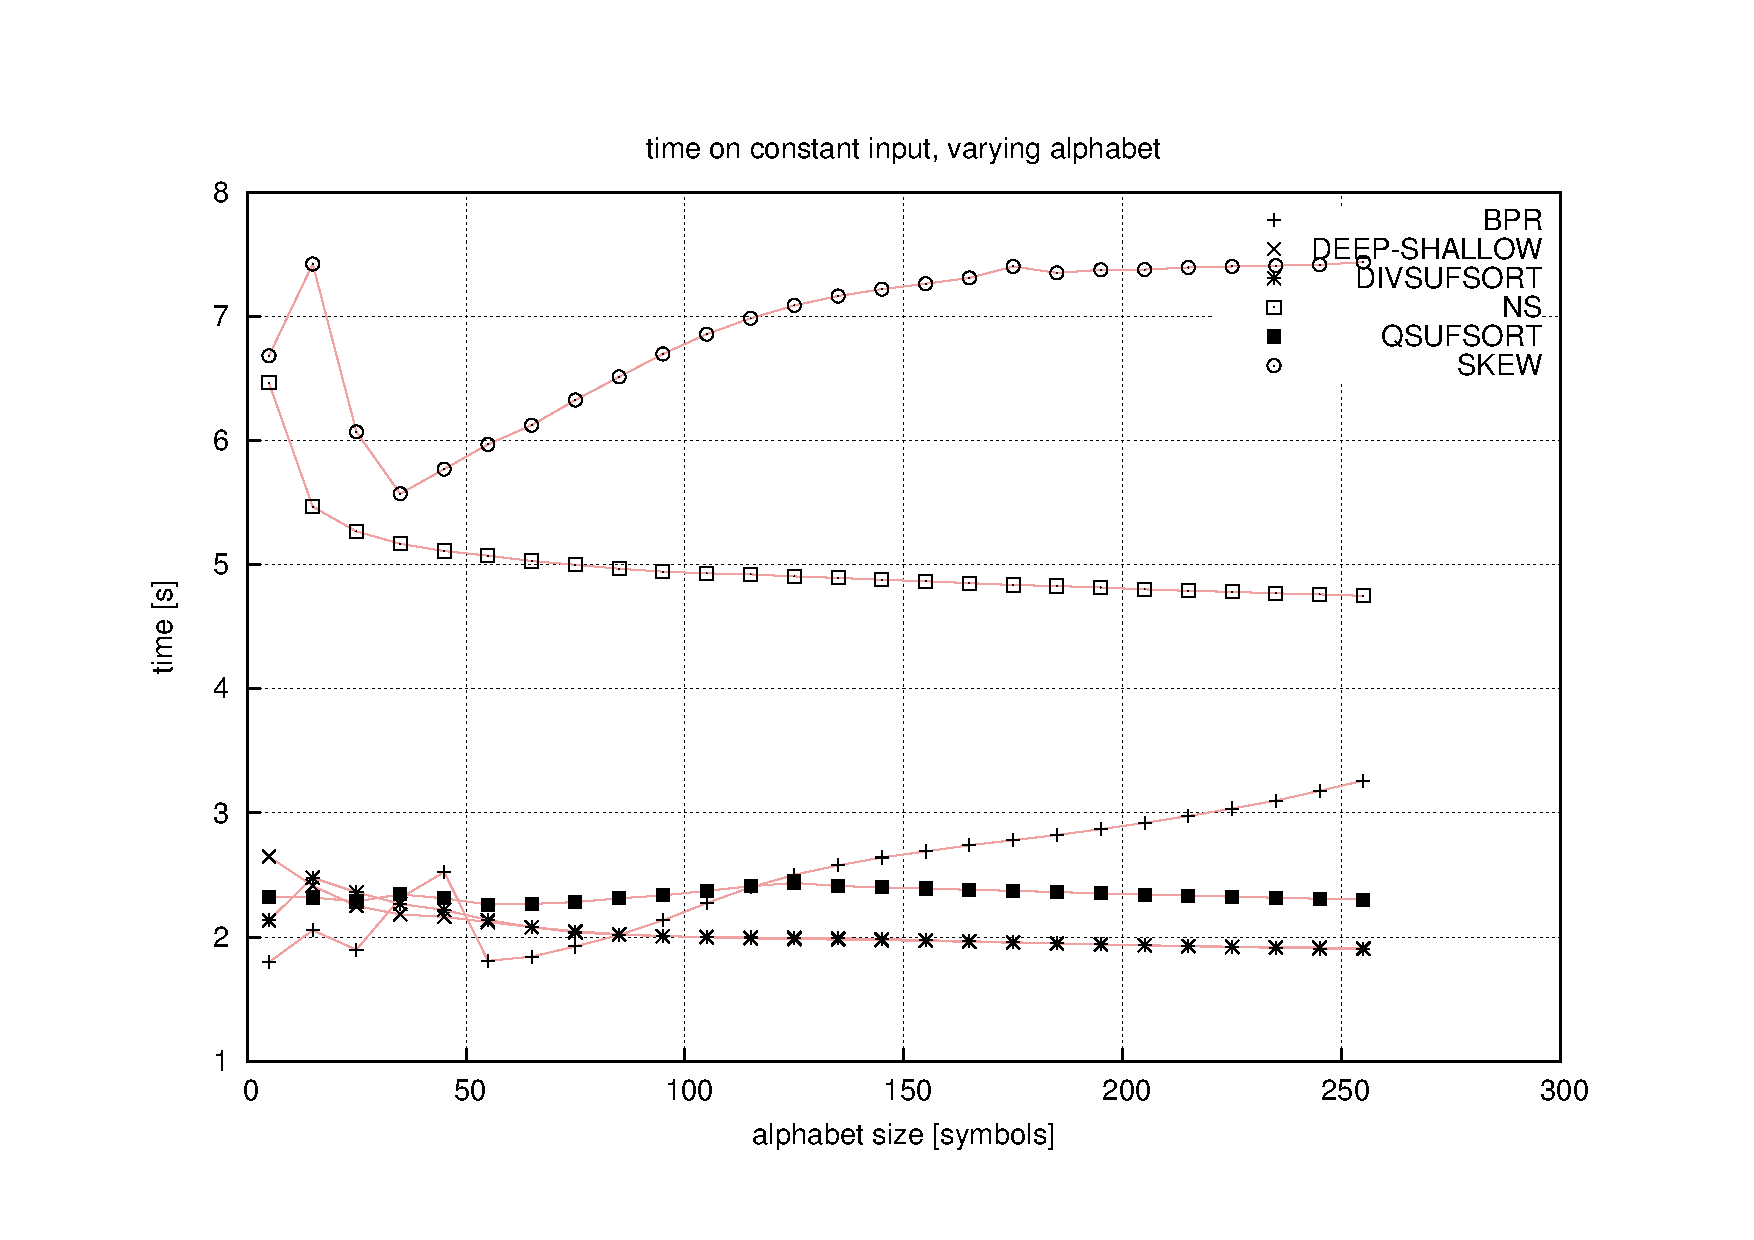
\includegraphics[width=\linewidth]{figures/results/random-alphabet-time.pdf}
        \end{center}        
    \caption{Czas działania algorytmów w~zależności od wielkości alfabetu.}%
    \label{rys:random-alphabet-time}
\end{figure}


% Flush manually before the main section.
\FloatBarrier

\section{Testy wydajnościowe na wejściu wczytywanym z~plików}

Zaimplementowane algorytmy przetestowane zostały na dwóch zestawach plików (korpusach) specjalnie
przygotowanych do testowania algorytmów tworzenia tablic sufiksów. Pierwszy z~nich nosi nazwę
\texttt{Gauntlet}, powstał z~inicjatywy Michaela Maniscalco. Ideą stojącą za stworzeniem tego
korpusu było zebranie plików o~nietypowej strukturze w~celu testowania algorytmów na szczególnych
przypadkach wejścia. Wkład w~powstanie tego zbioru plików wnieśli Yuta Mori, Simon Puglisi oraz
Graham Houston. Korpus dostępny jest do pobrania pod adresem [\ref{gauntlet}].

Drugi korpus testowy opracowany został przez Giovanniego Manziniego. W~jego skład wchodzą
rzeczywiste pliki o~dużym rozmiarze pochodzące z~różnych źródeł. Zestaw plików dostępny jest do
pobrania pod adresem [\ref{manzini-corpus}]. Tabela \ref{tab:manzini-files} prezentuje
charakterystykę plików obu korpusów.

\begin{table}[ht]
    \begin{center} \small
    \begin{tabular}{l r r}
    \toprule
    Plik                    & Rozmiar           & Średnie \emph{lcp} \\ \midrule
    \texttt{abac}           &          200\,000 &         99\,997 \\         
    \texttt{abba}           &      10\,500\,600 &     2\,773\,939 \\         
    \texttt{book1x20}       &      15\,375\,420 &     6\,938\,159 \\         
    \texttt{fib\_s14930352} &      14\,930\,352 &     3\,940\,597 \\         
    \texttt{fss10}          &      12\,078\,908 &     2\,454\,179 \\         
    \texttt{fss9}           &       2\,851\,443 &        579\,353 \\         
    \texttt{houston}        &       3\,840\,000 &         52\,083 \\         
    \texttt{paper5x80}      &          981\,924 &        239\,421 \\         
    \texttt{test1}          &       2\,097\,152 &     1\,048\,064 \\         
    \texttt{test2}          &       2\,097\,152 &     1\,048\,064 \\         
    \texttt{test3}          &       2\,097\,152 &        984\,064 \\         
    \bottomrule
    \end{tabular}
    \hspace{1cm}
    \begin{tabular}{l r r}
    \toprule
    Plik                     & Rozmiar           & Średnie \emph{lcp} \\ \midrule
    \texttt{chr22.dna}       &      34\,553\,758 &          1\,979 \\         
    \texttt{etext99}         &     105\,277\,340 &          1\,108 \\         
    \texttt{gcc-3.0.tar}     &      86\,630\,400 &          8\,603 \\         
    \texttt{howto}           &      39\,422\,105 &             267 \\         
    \texttt{jdk13c}          &      69\,728\,899 &             678 \\         
    \texttt{linux-2.4.5.tar} &     116\,254\,720 &             479 \\         
    \texttt{rctail96}        &     114\,711\,151 &             282 \\         
    \texttt{rfc}             &     116\,421\,901 &              93 \\         
    \texttt{sprot34.dat}     &     109\,617\,186 &              89 \\         
    \texttt{w3c2}            &     104\,201\,579 &         42\,299 \\
    \bottomrule
    \\
    \end{tabular}
    
    \end{center}                         
    \caption{Charakterystyka plików wchodzących w~skład korpusu \texttt{Gauntlet}
    (po lewej) i~korpusu Giovanniego Manziniego (po prawej). Rozmiar i~średnie \emph{lcp} podano w bajtach.}%
    \label{tab:gauntlet-files}\label{tab:manzini-files}
\end{table}


\subsection{Szczegółowe wyniki na maszynie wirtualnej firmy Sun}
    
Ze względu na wysokie podobieństwo wyników, w~poniższym rozdziale prezentowane są szczegółowe
rezultaty tylko z~jednej maszyny wirtualnej (\texttt{sun}). Podobnie jak w~przypadku testów na
różnych komputerach, wyniki testów na różnych maszynach wirtualnych są identyczne w~sensie rankingu
algorytmów.
	
Algorytm \emph{deep-shallow} został pominięty w~poniższych testach ze względu na nieakceptowalnie długi
czas działania. Testy z~jego udziałem wykazały wielokrotnie gorszy czas działania algorytmu od
najgorszego z~pozostałych. Również ze względu na czas działania algorytmu pominięto metodę naiwną.
Algorytmy \emph{skew} i~\emph{bpr} podczas przetwarzania niektórych plików kończyły się wyjątkiem
braku pamięci. Takie przypadki oznaczone zostały w~zestawieniach znakiem --, błąd
działania algorytmu na jednym z~plików danego korpusu powodował pominięcie tej metody w~podsumowaniu
testów na całym zbiorze plików.
	
Wyniki testów na korpusie \texttt{The Gauntlet} przedstawione zostały w~tabeli
\ref{tab:sun-gauntlet}. Rysunek \ref{rys:sun-gauntlet} obrazuje porównanie sumy czasów działania
algorytmów na wszystkich plikach korpusu (poza tymi algorytmami, które błędnie zakończyły
działanie). Analogiczne wyniki testów na korpusie Giovanniego Manziniego przedstawione są w~tabeli
\ref{tab:sun-manzini} oraz rysunku \ref{rys:sun-manzini}. Najlepszym algorytmem okazał się być
\emph{qsufsort}, który uzyskał najlepszy wynik na znakomitej większości plików. Drugie miejsce
przypadło algorytmowi \emph{divsufsort}. Pozostałe algorytmy uzyskiwały znacznie gorsze wyniki lub
nie kończyły obliczeń.


\begin{table}[ht]
    \begin{center}        
        \begin{tabular}{l r r r r } \toprule
 & \emph{bpr} & \emph{divsufsort} & \emph{qsufsort} & \emph{skew}\\ \midrule
\texttt{abac} & 1.04 & 0.01 & \textbf{0.01} & 0.05\\
\texttt{abba} & 4.23 & \textbf{2.19} & 2.26 & 11.23\\
\texttt{book1x20} & \textbf{3.14} & 3.29 & 3.40 & 22.52\\
\texttt{fib\_s14930352} & 10.05 & 4.94 & \textbf{3.32} & 14.09\\
\texttt{fss10} & 5.36 & 3.88 & \textbf{2.69} & 12.34\\
\texttt{fss9} & 1.05 & 0.63 & \textbf{0.58} & 1.89\\
\texttt{houston} & 2.63 & \textbf{0.24} & 0.44 & 0.96\\
\texttt{paper5x80} & 0.18 & 0.15 & \textbf{0.08} & 0.42\\
\texttt{test1} & 2.26 & 0.41 & \textbf{0.20} & 1.91\\
\texttt{test2} & 0.71 & 0.34 & \textbf{0.20} & 1.91\\
\texttt{test3} & 74.40 & 0.42 & \textbf{0.37} & 0.91\\
 \midrule
Total & 105.05 & 16.49 & \textbf{13.55} & 68.24\\
 \bottomrule
\end{tabular}

    \end{center}                         
    \caption{Czas działania algorytmów na plikach z~korpusu \texttt{Gauntlet}.}%
    \label{tab:sun-gauntlet}
\end{table}

\begin{figure}[ht]
   \begin{center}
        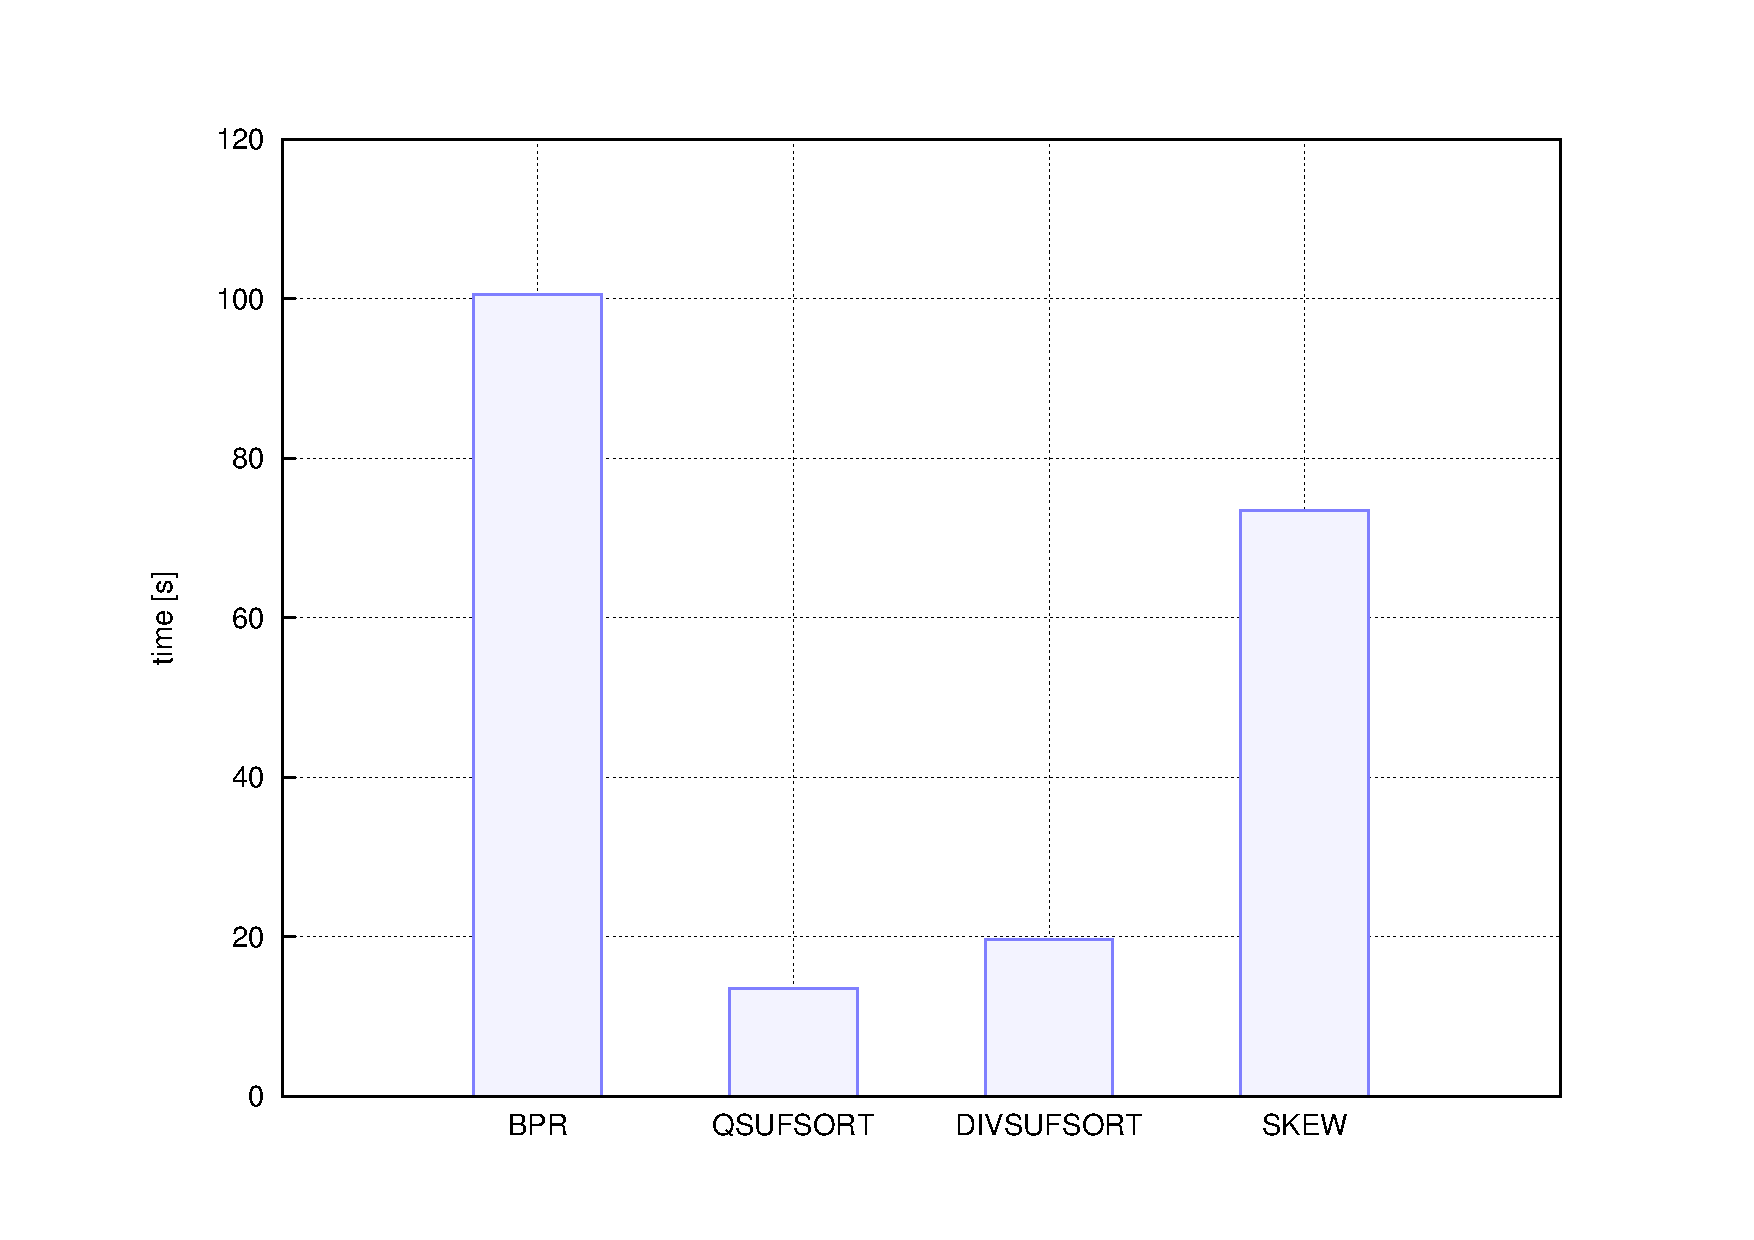
\includegraphics[width=\linewidth]{figures/results/sun-gauntlet.pdf}
    \end{center}        
    \caption{Sumaryczny czas działania algorytmów na plikach z~korpusu \texttt{Gauntlet}.}%
    \label{rys:sun-gauntlet}
\end{figure} 

\begin{table}[ht]
    \begin{center}        
        \begin{tabular}{l r r r r } \toprule
 & \emph{bpr} & \emph{divsufsort} & \emph{qsufsort} & \emph{skew}\\ \midrule
\texttt{chr22.dna} & \textbf{7.93} & 9.15 & 8.38 & 63.94\\
\texttt{etext99} & 32.45 & 32.38 & \textbf{29.48} & ---\\
\texttt{gcc-3.0.tar} & 25.45 & 19.74 & \textbf{16.61} & ---\\
\texttt{howto} & 9.71 & 9.92 & \textbf{8.46} & 82.36\\
\texttt{jdk13c} & 18.77 & 16.84 & \textbf{13.59} & ---\\
\texttt{linux-2.4.5.tar} & 29.32 & 27.61 & \textbf{24.55} & ---\\
\texttt{rctail96} & 35.18 & 32.71 & \textbf{27.64} & ---\\
\texttt{rfc} & 32.69 & 29.21 & \textbf{28.99} & ---\\
\texttt{sprot34.dat} & 32.81 & 31.97 & \textbf{25.60} & ---\\
\texttt{w3c2} & 27.51 & 25.63 & \textbf{20.47} & ---\\
 \midrule
Total & 251.82 & 235.16 & \textbf{203.76} & \\
 \bottomrule
\end{tabular}
 
    \end{center}                         
    \caption{Czas działania algorytmów na plikach z~korpusu Giovanniego Manziniego.}%
    \label{tab:sun-manzini}
\end{table}

\begin{figure}[ht]
   \begin{center}
        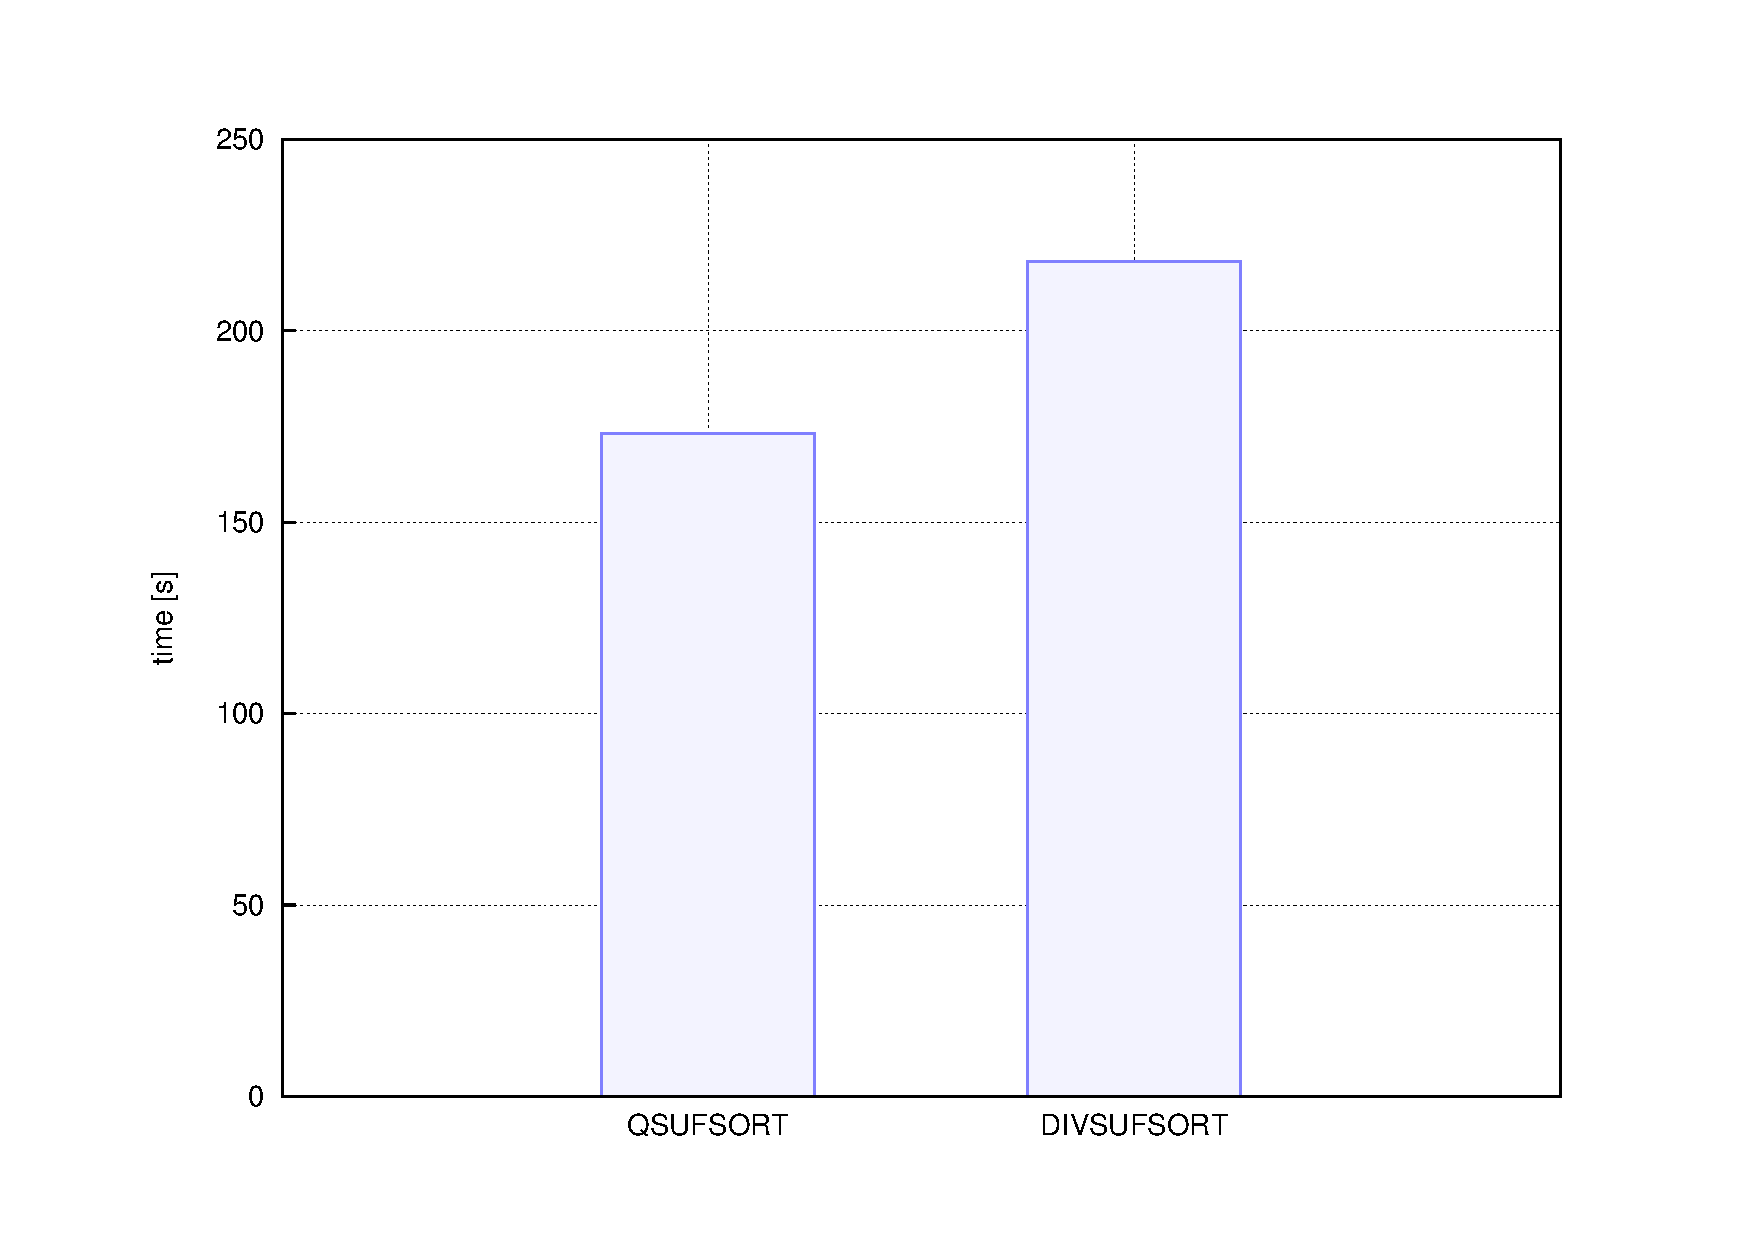
\includegraphics[width=\linewidth]{figures/results/sun-manzini.pdf}
    \end{center}        
    \caption{Sumaryczny czas działania algorytmów na plikach z~korpusu Giovanniego Manziniego.}%
    \label{rys:sun-manzini}
\end{figure} 


\FloatBarrier
\subsection{Porównanie czasów działania algorytmów na różnych maszynach wirtualnych}\label{sect:vms}

Poniżej przedstawione są wyniki podsumowań czasów działania algorytmów na korpusach testowych. Jak
już wspomniano wcześniej, ranking algorytmów jest identyczny dla każdej maszyny wirtualnej. Celem
prezentowania zestawień jest znalezienie takiej maszyny wirtualnej, na której algorytmy działają
najszybciej. Tabele \ref{tab:manzini-vm-compare} i~\ref{tab:gauntlet-vm-compare} zawierają czasy
działań algorytmów na plikach z~korpusów Giovanniego Manziniego i~\texttt{The Gauntlet}. Ze względu
na bardzo niskie wartości odchylenia standardowego nie umieszczono go tabelach. Wizualne porównanie
sum tych wyników znajduje się na rysunkach \ref{rys:manzini-vm-compare}
i~\ref{rys:gauntlet-vm-compare}.
	
Testowane maszyny wirtualne wypadły bardzo podobnie. Na maszynie \texttt{harmony} algorytmy działały
wolniej, wyniki pozostałych trzech maszyn są do siebie zbliżone. Spośród tych wyników wyróżnia się
jednak wynik testu algorytmu \emph{divsufsort} na korpusie Manziniego przeprowadzonego na maszynie
wirtualnej \texttt{jrockit} -- dwukrotnie gorszy niż na pozostałych maszynach. Wyniki w~tabeli
\ref{tab:jrockit-manzini} pokazują wolniejsze działania algorytmu na każdym z~plików wejściowych.
Analiza zapisów przebiegu działania algorytmu wykazała bardzo duże odchylenie standardowe czasu
działania algorytmu, co sugeruje wpływ maszyny wirtualnej (\emph{JIT}, \emph{garbage
collector}) lub jakiś inny proces obliczeniowy działające w tle i~zaburzający pomiar czasu.

\begin{table}[ht]
    \begin{center}        
        \begin{tabular}{l r r r r } \toprule
 & \emph{bpr} & \emph{divsufsort} & \emph{qsufsort} & \emph{skew} \\ \midrule
\texttt{sun} & 100.58 & 19.70 & 13.55 & 73.44 \\
\texttt{ibm} & --- & 18.49 & 14.71 & 71.02 \\
\texttt{jrockit} & 105.05 & 16.49 & 13.55 & 68.24 \\
\texttt{harmony} & 126.39 & 20.85 & 16.51 & 72.53 \\
\bottomrule
\end{tabular}
 
    \end{center}                         
    \caption{Czasy działania algorytmów na korpusie \texttt{Gauntlet} na różnych maszynach wirtualnych. Podane wartości wyrażone są w~sekundach.}
    \label{tab:gauntlet-vm-compare}
\end{table}

\begin{table}[ht]
    \begin{center}        
        \begin{tabular}{l r r r } \toprule
 & \emph{bpr} & \emph{divsufsort} & \emph{qsufsort} \\ \midrule
\texttt{sun} & --- & 218.09 & 173.10  \\
\texttt{ibm} & --- & 212.62 & 179.12 \\
\texttt{jrockit} & 200.84 & 416.30 & 170.00 \\
\texttt{harmony} & 251.82 & 235.16 & 203.76 \\
\bottomrule
\end{tabular}

 
    \end{center}                         
    \caption{Czasy działania algorytmów na korpusie Giovanniego Manziniego na różnych maszynach wirtualnych. Podane wartości wyrażone są w~sekundach.}
    \label{tab:manzini-vm-compare}
\end{table}

% TODO: kolorowe rysunki nie są dobrym pomysłem na wydruk, a te wszystkie kolory są tak samo pastelowe i wyjdą szaro. No
% chyba, że będziesz drukował w kolorze...

\begin{figure}[p]
    \begin{center}
        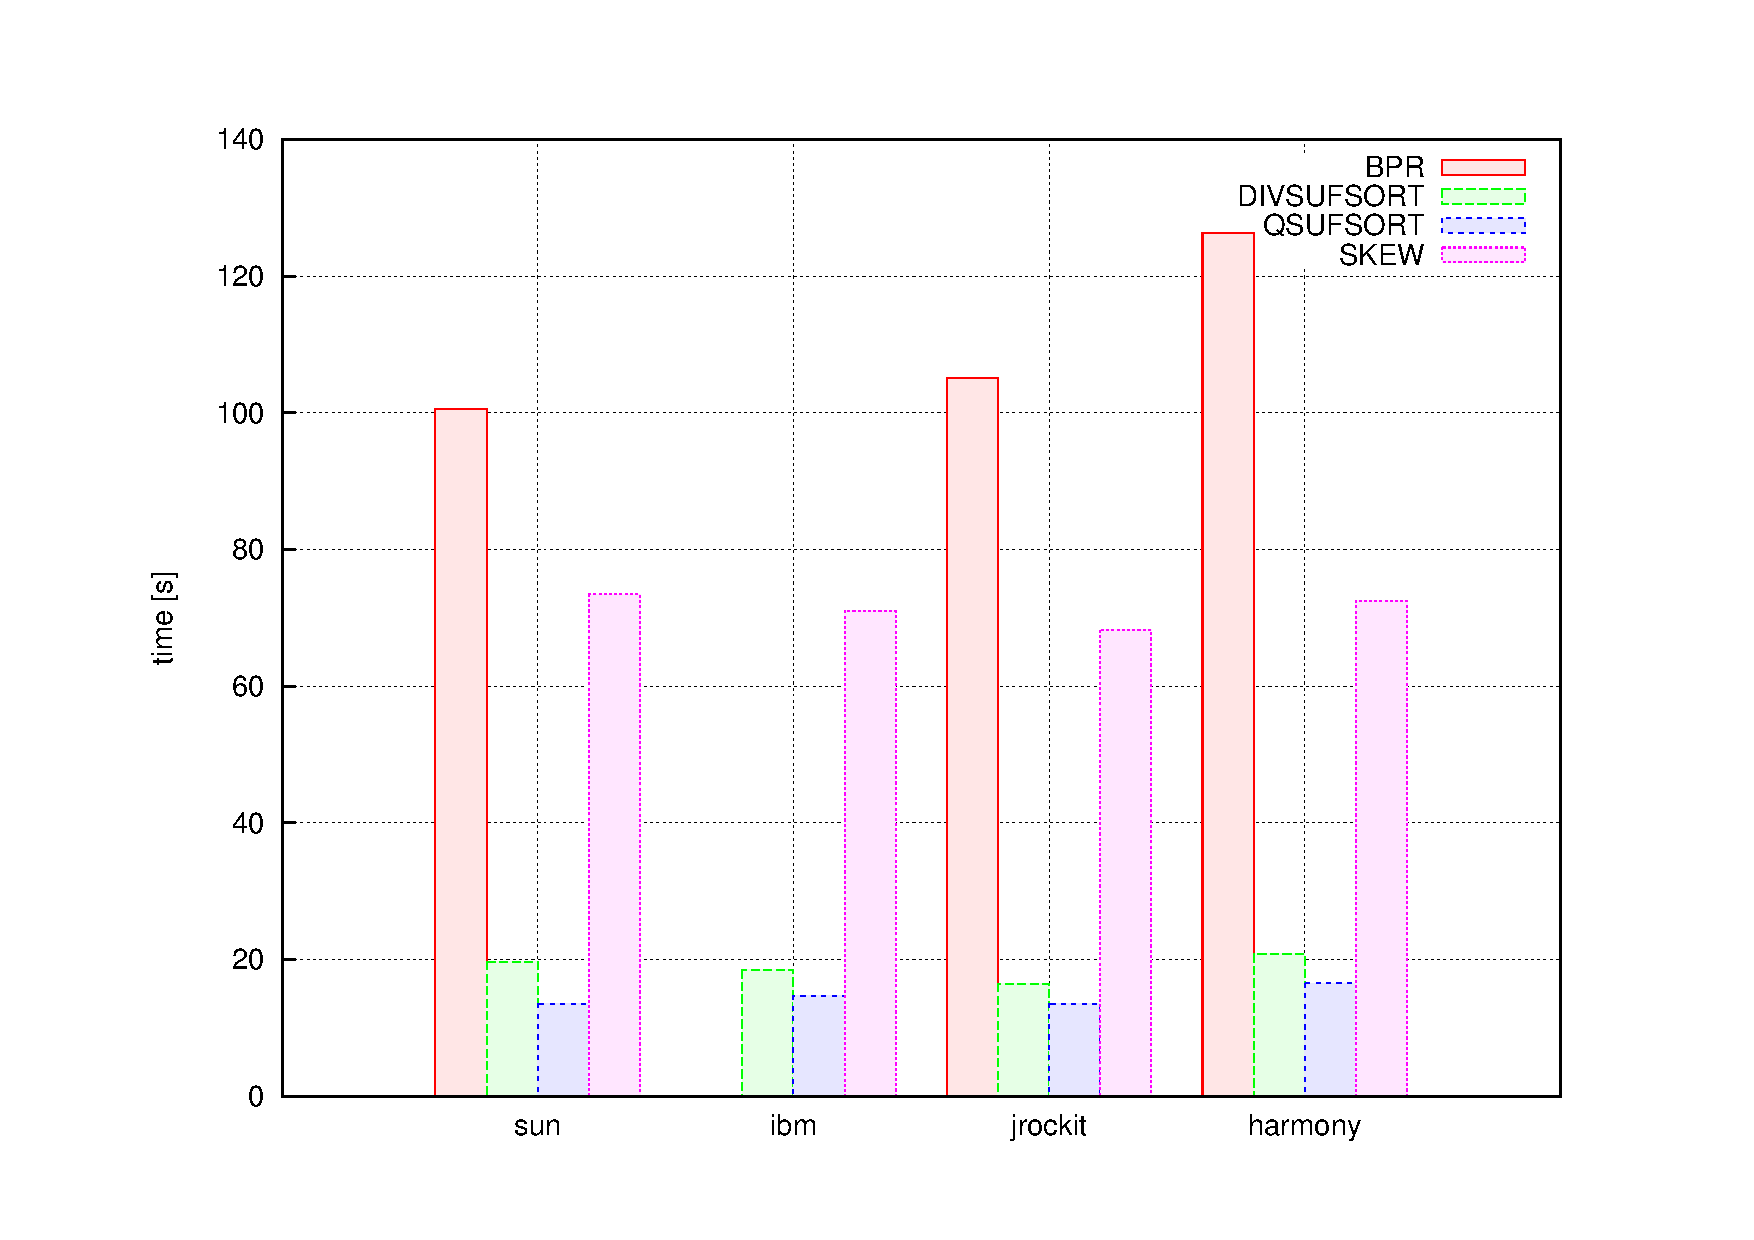
\includegraphics[width=.9\linewidth]{figures/results/gauntlet-compare.pdf}
    \end{center}        
    \caption{Porównanie czasu działania algorytmów na korpusie \texttt{Gauntlet} na różnych maszynach wirtualnych.}
    \label{rys:gauntlet-vm-compare}
\end{figure}

\begin{figure}[p]
    \begin{center}
        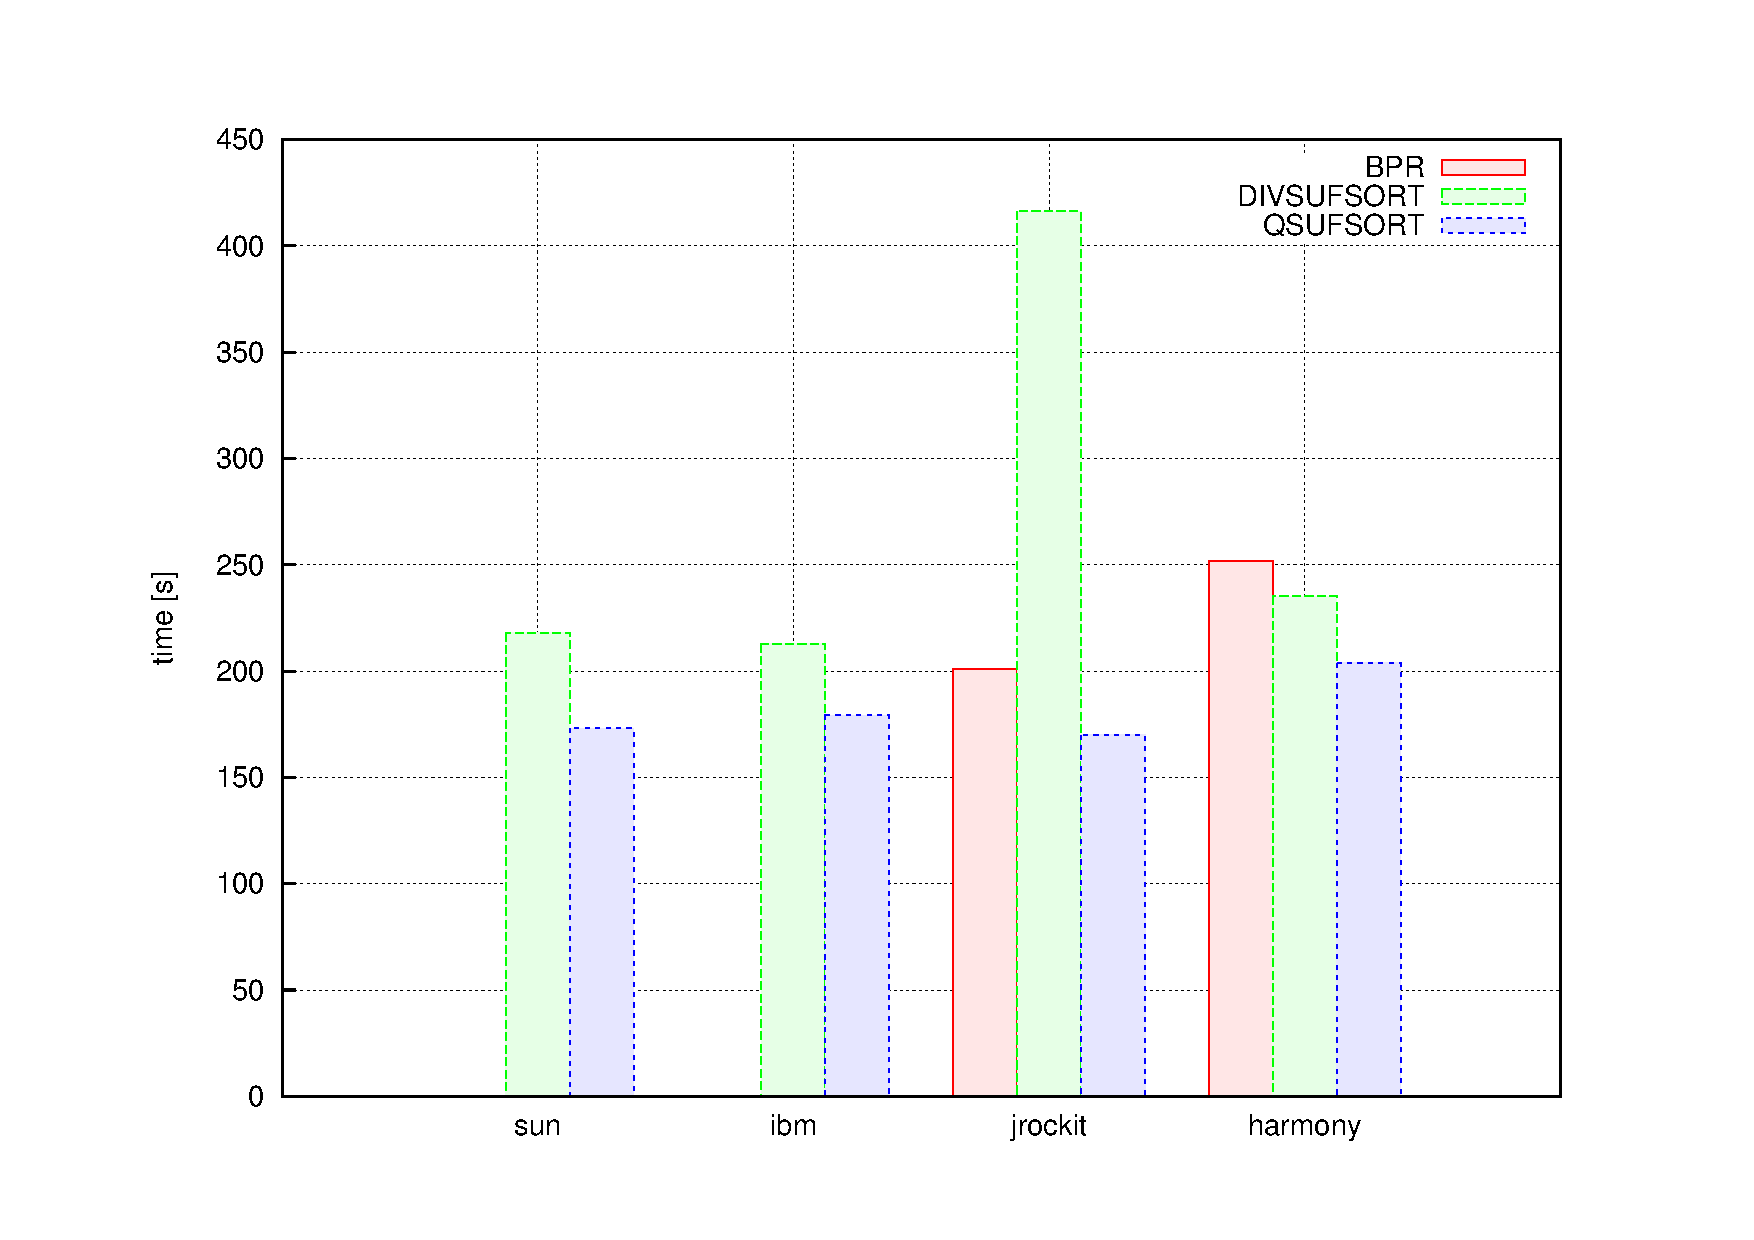
\includegraphics[width=.9\linewidth]{figures/results/manzini-compare.pdf}
        \end{center}        
        \caption{Porównanie czasu działania algorytmów na korpusie Giovanniego Manziniego na różnych maszynach wirtualnych.}
        \label{rys:manzini-vm-compare}
\end{figure}


\FloatBarrier
\section{Analiza wyników}

Najlepszym spośród zaimplementowanych algorytmów okazał się algorytm \emph{qsufsort}. Cechuje się on
odpornością na specyficzne typy danych wejściowych, nie zależy w dużym stopniu ani od rozmiaru
alfabetu sekwencji wejściowej ani od wartości średniego \emph{lcp}. Dodatkowym atutem jest brak
użycia dodatkowej pamięci ponad tą wymaganą do przechowania wejścia i~wyjścia algorytmu (oraz stosu
zużytego podczas rekurencyjnego sortowania). Na drugim miejscu znalazł się algorytm
\emph{divsufsort} ustępujący zwycięzcy zarówno pod względem czasu działania, jak i~zużycia pamięci.
Pozostałe algorytmy wypadły dużo gorzej niż wymieniona dwójka.

Co ciekawe, publikowane w~internecie wyniki testów wydajnościowych implementacji algorytmów w~języku
\texttt{C++} [\ref{msufsort}, \ref{mori-benchmark}] dają nieco inny obraz rankingu tych algorytmów.
Najlepsze wyniki uzyskują tam implementacje algorytmu \emph{improved two-stage}, czyli
\emph{archon}, \emph{divsufsort} i~\emph{msufsort}. Algorytm \emph{qsufsort} uzyskuje dobre, choć
wyraźnie gorsze wyniki. Wytłumaczenie przyczyn tego faktu leży zapewne w~różnicach między językami
\texttt{C++} a~\texttt{Java} (oraz działaniem kodu natywnego i~kodu uruchamianego na maszynie
wirtualnej). Algorytm \emph{qsufsort} jest prostym algorytmem, zarówno koncepcyjnie jak
i~implementacyjnie. Przepisanie go z~\texttt{C++} do \texttt{Javy} nie było trudne. Algorytm
\emph{divsufsort} jest dużo bardziej złożony (jego implementacja w~języku \texttt{Java} jest o~ponad
2000 linii kodu dłuższa od \emph{qsufsort}). Z~powodu wykorzystywania wskaźników oraz instrukcji
\texttt{\#define} w~oryginalnej implementacji, kod w~języku \texttt{Java} różni się od oryginału
w~wielu miejscach. Wydaje się, że dominujące dla szybkości działania różnice to:
\begin{itemize}
    \item allokacja złożonych struktur danych (i tablic lokalnych) następuję w języku \texttt{Java}
    na stercie, a nie na stosie; oprócz samego narzutu allokacji dochodzi tu również koszt 
    procesu oczyszczania pamięci (\emph{garbage collector});
    
    \item wskaźniki z języków niskopoziomowych muszą być modelowane jako indeksy nad tablicami typów prostych, 
    co w języku \texttt{Java} wiąże się z dodatkowym narzutem sprawdzenia czy indeks nie przekracza
    rozmiaru tablicy;

    \item rozmiar kodu natywnego generowanego dynamicznie w języku \texttt{Java} prawdopodobnie przekraczał wielokrotnie
    rozmiar kodu skompilowanego w języku \texttt{C}, powodując gorsze użytkowanie pamięci podręcznej
    procesora.
\end{itemize}

Algorytm \emph{skew} jako jedyny spośród testowanych algorytmów posiadał liniową teoretyczną złożoność
obliczeniową. W~testach wydajnościowych wypadł jednak bardzo słabo, zarówno w~testach implementacji
w~języku \texttt{Java}, jak i~w~języku \texttt{C++}. Przyczyną takiego zachowania algorytmu jest
jego bardzo duża złożoność pamięciowa zwiększana dodatkowo przez rekurencyjne wywoływanie algorytmu.
Ponadto, rekurencja wiąże się z~dodatkowymi kosztami związanymi z~obsługą stosu. Należy również
pamiętać, że podane złożoności pozostałych algorytmów są wartościami pesymistycznymi, które są
rzadko osiągane w praktyce.


